%!TEX encoding = UTF-8 Unicode

\documentclass[journal]{IEEEtran}

\usepackage[T1]{fontenc} % output - specifies encoding used in fonts; needs full LaTeX distribution to produce good-looking output
\usepackage[utf8]{inputenc} % input - type accented characters directly from keyboard
\usepackage[english]{babel} % internationalization - hyphenation, typographic rules for one or more languages

\usepackage[
    backend=biber, % bibliography engine
    style=ieee, % bibliography style .bbx and citation style .cbx
    hyperref, % make citations and references clickable - requires hyperref pkg
    maxbibnames=99, % 99 = display all authors of multi-author articles
    doi=false, % do not display DOI
    isbn=false, % do not display ISBN
    ]
        {biblatex} % note: incompatible with ucs (-> utf8x), natbib
\usepackage[
    autostyle] % adapt citation style to current document language
        {csquotes} % Context Sensitive Quotations; provides biblatex \enquote{}

\usepackage[nolist]{acronym}
\usepackage{amsmath}
\usepackage{amssymb}
\usepackage{booktabs}
\usepackage{graphicx}
\usepackage{hyperref}
\usepackage{subfig}
\usepackage{tabularx}
\usepackage{url}

\usepackage{tikz}
\usetikzlibrary{matrix,positioning}
\usetikzlibrary{decorations.text}
\usetikzlibrary{shapes.geometric}
\usetikzlibrary{fit}
\tikzstyle{circle}=[shape=circle,minimum size=0.7cm,very thick]
\tikzstyle{every path}=[very thick]
% https://tex.stackexchange.com/a/80090/18819
% TODO: after upgrading to TikZ 3.0+, use arrows.meta
\usetikzlibrary{arrows}
% This is not an official TikZ library. Use at your own risk!

\makeatletter
% alternative latex arrow
\pgfarrowsdeclare{latexnew}{latexnew}
{
  \ifdim\pgfgetarrowoptions{latexnew}=-1pt%
    \pgfutil@tempdima=0.28pt%
    \pgfutil@tempdimb=\pgflinewidth%
    \ifdim\pgfinnerlinewidth>0pt%
      \pgfmathsetlength\pgfutil@tempdimb{.6\pgflinewidth-.4*\pgfinnerlinewidth}%
    \fi%
    \advance\pgfutil@tempdima by.3\pgfutil@tempdimb%
  \else%
    \pgfutil@tempdima=\pgfgetarrowoptions{latexnew}%
    \divide\pgfutil@tempdima by 10%
  \fi%
  \pgfarrowsleftextend{+-1\pgfutil@tempdima}%
  \pgfarrowsrightextend{+9\pgfutil@tempdima}%
}
{
  \ifdim\pgfgetarrowoptions{latexnew}=-1pt%
    \pgfutil@tempdima=0.28pt%
    \pgfutil@tempdimb=\pgflinewidth%
    \ifdim\pgfinnerlinewidth>0pt%
      \pgfmathsetlength\pgfutil@tempdimb{.6\pgflinewidth-.4*\pgfinnerlinewidth}%
    \fi%
    \advance\pgfutil@tempdima by.3\pgfutil@tempdimb%
  \else%
    \pgfutil@tempdima=\pgfgetarrowoptions{latexnew}%
    \divide\pgfutil@tempdima by 10%
    \pgfsetlinewidth{0bp}%
  \fi%
  \pgfpathmoveto{\pgfqpoint{9\pgfutil@tempdima}{0pt}}
  \pgfpathcurveto
  {\pgfqpoint{6.3333\pgfutil@tempdima}{.5\pgfutil@tempdima}}
  {\pgfqpoint{2\pgfutil@tempdima}{2\pgfutil@tempdima}}
  {\pgfqpoint{-1\pgfutil@tempdima}{3.75\pgfutil@tempdima}}
  \pgfpathlineto{\pgfqpoint{-1\pgfutil@tempdima}{-3.75\pgfutil@tempdima}}
  \pgfpathcurveto
  {\pgfqpoint{2\pgfutil@tempdima}{-2\pgfutil@tempdima}}
  {\pgfqpoint{6.3333\pgfutil@tempdima}{-.5\pgfutil@tempdima}}
  {\pgfqpoint{9\pgfutil@tempdima}{0pt}}
  \pgfusepathqfill
}

% alternative latex reversed arrow
\pgfarrowsdeclarereversed{latexnew reversed}{latexnew reversed}{latexnew}{latexnew}

% alternative latex' arrow
\pgfarrowsdeclare{latex'new}{latex'new}
{
  \ifdim\pgfgetarrowoptions{latex'new}=-1pt%
    \pgfutil@tempdima=0.28pt%
    \advance\pgfutil@tempdima by.3\pgflinewidth%
  \else%
    \pgfutil@tempdima=\pgfgetarrowoptions{latex'new}%
    \divide\pgfutil@tempdima by 10%
  \fi%
  \pgfarrowsleftextend{+-4\pgfutil@tempdima}
  \pgfarrowsrightextend{+6\pgfutil@tempdima}
}
{
  \ifdim\pgfgetarrowoptions{latex'new}=-1pt%
    \pgfutil@tempdima=0.28pt%
    \advance\pgfutil@tempdima by.3\pgflinewidth%
  \else%
    \pgfutil@tempdima=\pgfgetarrowoptions{latex'new}%
    \divide\pgfutil@tempdima by 10%
    \pgfsetlinewidth{0bp}%
  \fi%
  \pgfpathmoveto{\pgfqpoint{6\pgfutil@tempdima}{0\pgfutil@tempdima}}
  \pgfpathcurveto
  {\pgfqpoint{3.5\pgfutil@tempdima}{.5\pgfutil@tempdima}}
  {\pgfqpoint{-1\pgfutil@tempdima}{1.5\pgfutil@tempdima}}
  {\pgfqpoint{-4\pgfutil@tempdima}{3.75\pgfutil@tempdima}}
  \pgfpathcurveto
  {\pgfqpoint{-1.5\pgfutil@tempdima}{1\pgfutil@tempdima}}
  {\pgfqpoint{-1.5\pgfutil@tempdima}{-1\pgfutil@tempdima}}
  {\pgfqpoint{-4\pgfutil@tempdima}{-3.75\pgfutil@tempdima}}
  \pgfpathcurveto
  {\pgfqpoint{-1\pgfutil@tempdima}{-1.5\pgfutil@tempdima}}
  {\pgfqpoint{3.5\pgfutil@tempdima}{-.5\pgfutil@tempdima}}
  {\pgfqpoint{6\pgfutil@tempdima}{0\pgfutil@tempdima}}
  \pgfusepathqfill
}

% alternative latex' reversed arrow
\pgfarrowsdeclarereversed{latex'new reversed}{latex'new reversed}{latex'new}{latex'new}

% alternative o arrow
\pgfarrowsdeclare{onew}{onew}
{
  \pgfarrowsleftextend{+-.5\pgflinewidth}
  \ifdim\pgfgetarrowoptions{onew}=-1pt%
    \pgfutil@tempdima=0.4pt%
    \advance\pgfutil@tempdima by.2\pgflinewidth%
    \pgfutil@tempdimb=9\pgfutil@tempdima\advance\pgfutil@tempdimb by.5\pgflinewidth%
    \pgfarrowsrightextend{+\pgfutil@tempdimb}%
  \else%
    \pgfutil@tempdima=\pgfgetarrowoptions{onew}%
    \advance\pgfutil@tempdima by -0.5\pgflinewidth%
    \pgfarrowsrightextend{+\pgfutil@tempdima}%
  \fi%
}
{ 
  \ifdim\pgfgetarrowoptions{onew}=-1pt%
    \pgfutil@tempdima=0.4pt%
    \advance\pgfutil@tempdima by.2\pgflinewidth%
    \pgfutil@tempdimb=0pt%
  \else%
    \pgfutil@tempdima=\pgfgetarrowoptions{onew}%
    \divide\pgfutil@tempdima by 9%
    \pgfutil@tempdimb=0.5\pgflinewidth%
  \fi%
  \pgfsetdash{}{+0pt}
  \pgfpathcircle{\pgfpointadd{\pgfqpoint{4.5\pgfutil@tempdima}{0bp}}%
                             {\pgfqpoint{-\pgfutil@tempdimb}{0bp}}}%
                {4.5\pgfutil@tempdima-\pgfutil@tempdimb}%
  \pgfusepathqstroke
}

% alternative square arrow
\pgfarrowsdeclare{squarenew}{squarenew}
{
 \ifdim\pgfgetarrowoptions{squarenew}=-1pt%
   \pgfutil@tempdima=0.4pt
   \advance\pgfutil@tempdima by.275\pgflinewidth%
   \pgfarrowsleftextend{+-\pgfutil@tempdima}
   \advance\pgfutil@tempdima by.5\pgflinewidth
   \pgfarrowsrightextend{+\pgfutil@tempdima}
 \else%
   \pgfutil@tempdima=\pgfgetarrowoptions{squarenew}%
   \divide\pgfutil@tempdima by 8%
   \pgfarrowsleftextend{+-7\pgfutil@tempdima}%
   \pgfarrowsrightextend{+1\pgfutil@tempdima}%
 \fi%
}
{
 \ifdim\pgfgetarrowoptions{squarenew}=-1pt%
   \pgfutil@tempdima=0.4pt%
   \advance\pgfutil@tempdima by.275\pgflinewidth%
   \pgfutil@tempdimb=0pt%
 \else%
   \pgfutil@tempdima=\pgfgetarrowoptions{squarenew}%   
   \divide\pgfutil@tempdima by 8%
   \pgfutil@tempdimb=0.5\pgflinewidth%
 \fi%
 \pgfsetdash{}{+0pt}
 \pgfsetroundjoin
 \pgfpathmoveto{\pgfpointadd{\pgfqpoint{1\pgfutil@tempdima}{4\pgfutil@tempdima}}
                            {\pgfqpoint{-\pgfutil@tempdimb}{-\pgfutil@tempdimb}}}
 \pgfpathlineto{\pgfpointadd{\pgfqpoint{-7\pgfutil@tempdima}{4\pgfutil@tempdima}}
                            {\pgfqpoint{\pgfutil@tempdimb}{-\pgfutil@tempdimb}}}
 \pgfpathlineto{\pgfpointadd{\pgfqpoint{-7\pgfutil@tempdima}{-4\pgfutil@tempdima}}
                            {\pgfqpoint{\pgfutil@tempdimb}{\pgfutil@tempdimb}}}
 \pgfpathlineto{\pgfpointadd{\pgfqpoint{1\pgfutil@tempdima}{-4\pgfutil@tempdima}}
                            {\pgfqpoint{-\pgfutil@tempdimb}{\pgfutil@tempdimb}}}
 \pgfpathclose
 \pgfusepathqfillstroke
}

% alternative stealth arrow
\pgfarrowsdeclare{stealthnew}{stealthnew}
{
  \ifdim\pgfgetarrowoptions{stealthnew}=-1pt%
    \pgfutil@tempdima=0.28pt%
    \pgfutil@tempdimb=\pgflinewidth%
    \ifdim\pgfinnerlinewidth>0pt%
      \pgfmathsetlength\pgfutil@tempdimb{.6\pgflinewidth-.4*\pgfinnerlinewidth}%
    \fi%
    \advance\pgfutil@tempdima by.3\pgfutil@tempdimb%
  \else%
    \pgfutil@tempdima=\pgfgetarrowoptions{stealthnew}%
    \divide\pgfutil@tempdima by 8%
  \fi%
  \pgfarrowsleftextend{+-3\pgfutil@tempdima}
  \pgfarrowsrightextend{+5\pgfutil@tempdima}
}
{
  \ifdim\pgfgetarrowoptions{stealthnew}=-1pt%
    \pgfutil@tempdima=0.28pt%
    \pgfutil@tempdimb=\pgflinewidth%
    \ifdim\pgfinnerlinewidth>0pt%
      \pgfmathsetlength\pgfutil@tempdimb{.6\pgflinewidth-.4*\pgfinnerlinewidth}%
    \fi%
    \advance\pgfutil@tempdima by.3\pgfutil@tempdimb%
  \else%
    \pgfutil@tempdima=\pgfgetarrowoptions{stealthnew}%
    \divide\pgfutil@tempdima by 8%
    \pgfsetlinewidth{0bp}%
  \fi%
  \pgfpathmoveto{\pgfqpoint{5\pgfutil@tempdima}{0pt}}
  \pgfpathlineto{\pgfqpoint{-3\pgfutil@tempdima}{4\pgfutil@tempdima}}
  \pgfpathlineto{\pgfpointorigin}
  \pgfpathlineto{\pgfqpoint{-3\pgfutil@tempdima}{-4\pgfutil@tempdima}}
  \pgfusepathqfill
}

% alternative stealth reversed arrow
\pgfarrowsdeclarereversed{stealthnew reversed}{stealthnew reversed}{stealthnew}{stealthnew}

% alternative to arrow
\pgfarrowsdeclare{tonew}{tonew}
{
  \ifdim\pgfgetarrowoptions{tonew}=-1pt%
    \pgfutil@tempdima=0.84pt%
    \advance\pgfutil@tempdima by1.3\pgflinewidth%
    \pgfutil@tempdimb=0.21pt%
    \advance\pgfutil@tempdimb by.625\pgflinewidth%
  \else%
    \pgfutil@tempdima=\pgfgetarrowoptions{tonew}%
    \pgfarrowsleftextend{+-0.8\pgfutil@tempdima}%
    \pgfarrowsrightextend{+0.2\pgfutil@tempdima}%
  \fi%
}
{
  \ifdim\pgfgetarrowoptions{tonew}=-1pt%
    \pgfutil@tempdima=0.28pt%
    \advance\pgfutil@tempdima by.3\pgflinewidth%
    \pgfutil@tempdimb=0pt,%
  \else%
    \pgfutil@tempdima=\pgfgetarrowoptions{tonew}%
    \multiply\pgfutil@tempdima by 100%
    \divide\pgfutil@tempdima by 375%
    \pgfutil@tempdimb=0.4\pgflinewidth%
  \fi%
  \pgfsetdash{}{+0pt}
  \pgfsetroundcap
  \pgfsetroundjoin
  \pgfpathmoveto{\pgfpointorigin}
  \pgflineto{\pgfpointadd{\pgfpoint{0.75\pgfutil@tempdima}{0bp}}
                         {\pgfqpoint{-2\pgfutil@tempdimb}{0bp}}}
  \pgfusepathqstroke
  \pgfsetlinewidth{0.8\pgflinewidth}
  \pgfpathmoveto{\pgfpointadd{\pgfqpoint{-3\pgfutil@tempdima}{4\pgfutil@tempdima}}
                             {\pgfqpoint{\pgfutil@tempdimb}{0bp}}}
  \pgfpathcurveto
  {\pgfpointadd{\pgfqpoint{-2.75\pgfutil@tempdima}{2.5\pgfutil@tempdima}}
               {\pgfqpoint{0.5\pgfutil@tempdimb}{0bp}}}
  {\pgfpointadd{\pgfqpoint{0pt}{0.25\pgfutil@tempdima}}
               {\pgfqpoint{-0.5\pgfutil@tempdimb}{0bp}}}
  {\pgfpointadd{\pgfqpoint{0.75\pgfutil@tempdima}{0pt}}
               {\pgfqpoint{-\pgfutil@tempdimb}{0bp}}}
  \pgfpathcurveto
  {\pgfpointadd{\pgfqpoint{0pt}{-0.25\pgfutil@tempdima}}
               {\pgfqpoint{-0.5\pgfutil@tempdimb}{0bp}}}
  {\pgfpointadd{\pgfqpoint{-2.75\pgfutil@tempdima}{-2.5\pgfutil@tempdima}}
               {\pgfqpoint{0.5\pgfutil@tempdimb}{0bp}}}
  {\pgfpointadd{\pgfqpoint{-3\pgfutil@tempdima}{-4\pgfutil@tempdima}}
               {\pgfqpoint{\pgfutil@tempdimb}{0bp}}}
  \pgfusepathqstroke
}

% alias alternative to arrow
\pgfarrowsdeclarealias{<new}{>new}{tonew}{tonew}

\makeatother

% tip length code
\pgfsetarrowoptions{latexnew}{-1pt}
\pgfsetarrowoptions{latex'new}{-1pt}
\pgfsetarrowoptions{onew}{-1pt}
\pgfsetarrowoptions{squarenew}{-1pt}
\pgfsetarrowoptions{stealthnew}{-1pt}
\pgfsetarrowoptions{tonew}{-1pt}
\pgfkeys{/tikz/.cd, arrowhead/.default=-1pt, arrowhead/.code={
  \pgfsetarrowoptions{latexnew}{#1},
  \pgfsetarrowoptions{latex'new}{#1},
  \pgfsetarrowoptions{onew}{#1},
  \pgfsetarrowoptions{squarenew}{#1},
  \pgfsetarrowoptions{stealthnew}{#1},
  \pgfsetarrowoptions{tonew}{#1},
}}

\tikzset{options/.code={\tikzset{#1}}} % just to compact the code
\tikzstyle{myarrow}=[->new, thick, arrowhead=0.2cm]


\usepackage{hyperref}
\usepackage[update,prepend]{epstopdf}
\graphicspath{{figures/}}

\addbibresource{lang_journal_bibliography.bib}

% custom commands and frequent expressions that require typesetting care
\newcommand{\AffWords}{Affordance--Words}
\newcommand{\affwords}{affordance--words}
\newcommand{\FB}{Forward--Backward}
\newcommand{\HR}{Human--Robot}
\newcommand{\HRI}{\HR{} Interaction}
\newcommand{\hh}{human--human}
\newcommand{\hr}{human--robot}
\newcommand{\hri}{\hr{} interaction}
\newcommand{\ObjAct}{Object--Action}
\newcommand{\SensMot}{Sensory--Motor}

\newcommand{\phmm}{\ensuremath{P_{\text{HMM}}}}
\newcommand{\pbn}{\ensuremath{P_{\text{BN}}}}
\newcommand{\pcomb}{\ensuremath{P_\text{comb}}}
\newcommand{\xinf}{\ensuremath{X_\text{inf}}}
\newcommand{\xobs}{\ensuremath{X_\text{obs}}}
\newcommand{\xlat}{\ensuremath{X_\text{lat}}}

%\newcommand{\given}{\ensuremath{|}} % Giampiero, without space around bar
\newcommand{\given}{\ensuremath{\mid}} % Giovanni, with space around bar

% list of acronyms
\begin{acronym}
\acro{AI}{Artificial Intelligence}
\acro{BN}{Bayesian Network}
\acro{HMM}{Hidden Markov Model}
\acro{MTRNN}{Multiple Timescales Recurrent Neural Network}
\acro{OAC}{\ObjAct{} Complex}
\acrodefplural{OAC}{\ObjAct{} Complexes}
\acro{PDF}{Probability Density Function}
\end{acronym}

%%%%%%%%%%%%%%%%%%%%%%%%%%%%%%%%%%%%%%%%%%%%%%%%%%%%%%%%%%%%%%%%%%%%%%%%%%%%%%%%
\begin{document}

\title{Beyond the Self: Using Grounded Affordance Knowledge to Interpret Others' Actions}

\author{Giovanni~Saponaro,~\IEEEmembership{Student Member,~IEEE,}
        Lorenzo~Jamone,~\IEEEmembership{Member,~IEEE,}
        Alexandre~Bernardino,~\IEEEmembership{Member,~IEEE}
        Giampiero~Salvi,~\IEEEmembership{Member,~IEEE}
\thanks{G.~Saponaro, and A.~Bernardino are with the
Institute for Systems and Robotics, Instituto Superior Técnico,
Universidade de Lisboa, Lisbon, Portugal, e-mail: \{gsaponaro,alex\}@isr.tecnico.ulisboa.pt.

L.~Jamone is with ARQ~(Advanced Robotics at Queen Mary), School of Electronic Engineering and Computer Science, Queen Mary University of London, United Kingdom
and with the
Institute for Systems and Robotics, Instituto Superior Técnico, Universidade de Lisboa, Lisbon, Portugal,
e-mail: l.jamone@qmul.ac.uk.

G.~Salvi is with the Speech, Music and Hearing Department,
KTH Royal Institute of Technology, Stockholm, Sweden,
e-mail: giampi@kth.se.
}}

% make the title area
\maketitle

%%%%%%%%%%%%%%%%%%%%%%%%%%%%%%%%%%%%%%%%%%%%%%%%%%%%%%%%%%%%%%%%%%%%%%%%%%%%%%%%
\begin{abstract}
TODO
\end{abstract}

\begin{IEEEkeywords}
affordances, gestures, humanoid robots, language learning.
\end{IEEEkeywords}

%%%%%%%%%%%%%%%%%%%%%%%%%%%%%%%%%%%%%%%%%%%%%%%%%%%%%%%%%%%%%%%%%%%%%%%%%%%%%%%%
%!TEX encoding = UTF-8 Unicode

\section{Introduction}

\newcommand{\myWidth}{0.22}

\begin{figure*}
    \centering
    \subfloat
    { 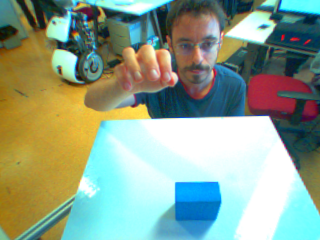
\includegraphics[width=\myWidth\linewidth]{grasp-00000169} } \quad
    %
    \subfloat
    { 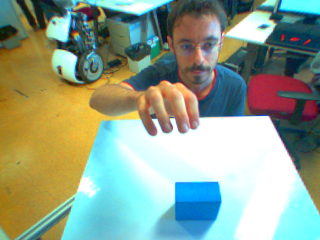
\includegraphics[width=\myWidth\linewidth]{grasp-00000170} } \quad
    %
    \subfloat
    { 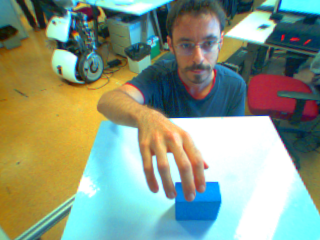
\includegraphics[width=\myWidth\linewidth]{grasp-00000171} } \\
    %
    \subfloat
    { 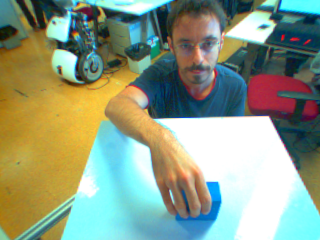
\includegraphics[width=\myWidth\linewidth]{grasp-00000173} } \quad
    %
    \subfloat
    { 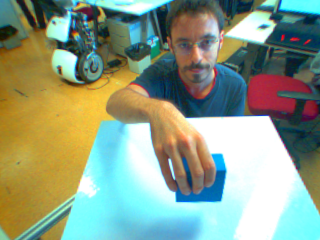
\includegraphics[width=\myWidth\linewidth]{grasp-00000177} } \quad
    %
    \subfloat
    { 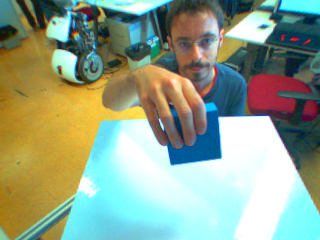
\includegraphics[width=\myWidth\linewidth]{grasp-00000180} }
    \caption{Grasp action example, from the point of view of the robot. An agent~(human) moves the hand towards an object vertically, then grasps and lifts it.}
\end{figure*}

\begin{figure*}
    \centering
    \subfloat
    { 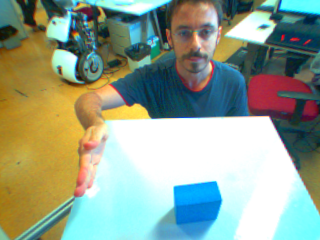
\includegraphics[width=\myWidth\linewidth]{tap-00000109} } \quad
    %
    \subfloat
    { 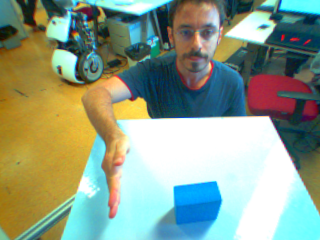
\includegraphics[width=\myWidth\linewidth]{tap-00000110} } \quad
    %
    \subfloat
    { 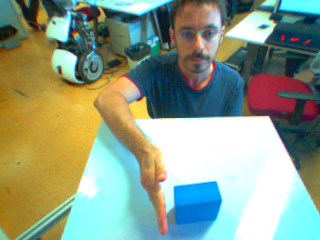
\includegraphics[width=\myWidth\linewidth]{tap-00000112} } \\
    %
    \subfloat
    { 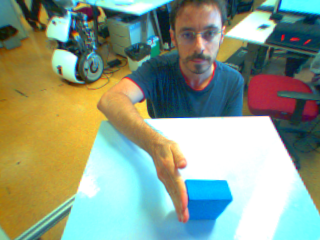
\includegraphics[width=\myWidth\linewidth]{tap-00000114} } \quad
    %
    \subfloat
    { 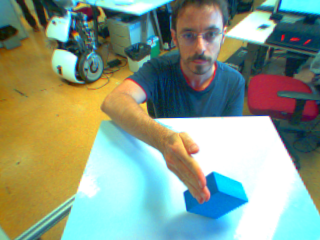
\includegraphics[width=\myWidth\linewidth]{tap-00000116} } \quad
    %
    \subfloat
    { 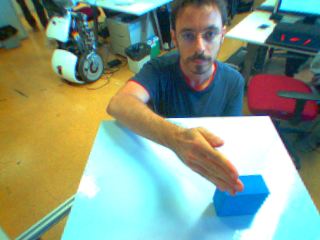
\includegraphics[width=\myWidth\linewidth]{tap-00000117} }
    \caption{Tap action example, from the point of view of the robot. An agent~(human) moves the hand towards an object laterally and touches it, causing a motion effect.}
\end{figure*}

\begin{figure*}
    \centering
    \subfloat
    { 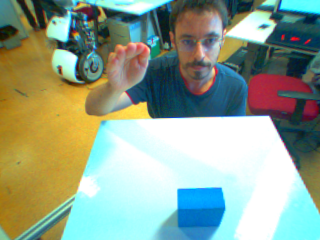
\includegraphics[width=\myWidth\linewidth]{touch-00000196} } \quad
    %
    \subfloat
    { 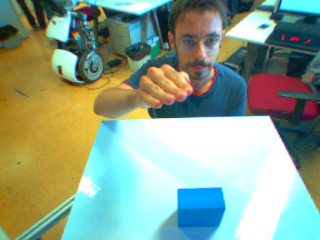
\includegraphics[width=\myWidth\linewidth]{touch-00000197} } \quad
    %
    \subfloat
    { 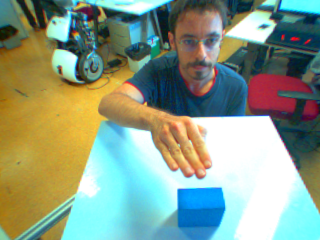
\includegraphics[width=\myWidth\linewidth]{touch-00000198} } \\
    %
    \subfloat
    { 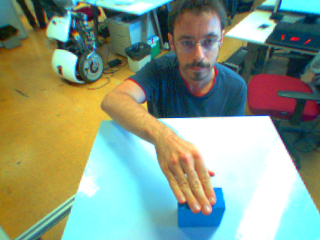
\includegraphics[width=\myWidth\linewidth]{touch-00000200} } \quad
    %
    \subfloat
    { 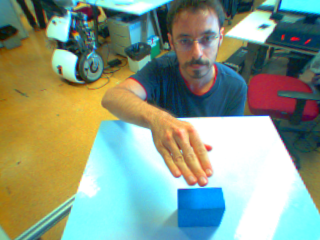
\includegraphics[width=\myWidth\linewidth]{touch-00000202} } \quad
    %
    \subfloat
    { 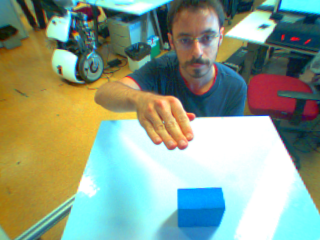
\includegraphics[width=\myWidth\linewidth]{touch-00000203} }
    \caption{Touch action example, from the point of view of the robot. An agent~(human) moves the hand towards an object vertically, then touches it~(without grasping), then retracts the hand.}
\end{figure*}

% TODO: delete the seq2-* png files (view from external camera)
% \begin{figure*}
%     \centering
%     \subfloat
%     { 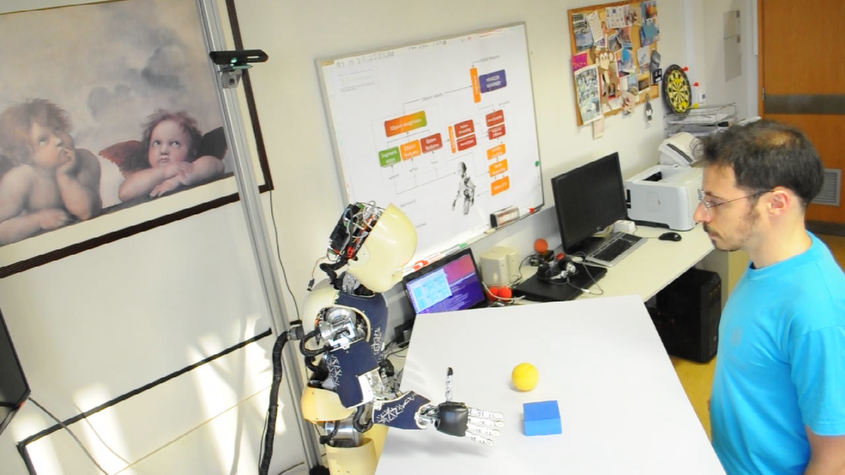
\includegraphics[width=\myWidth\linewidth]{seq2-grasp-11} } \quad
%     %
%     \subfloat
%     { 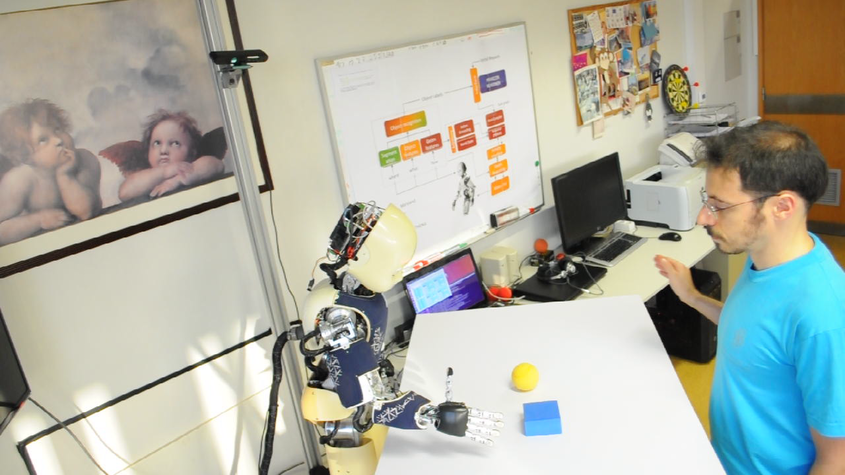
\includegraphics[width=\myWidth\linewidth]{seq2-grasp-12} } \quad
%     %
%     \subfloat
%     { 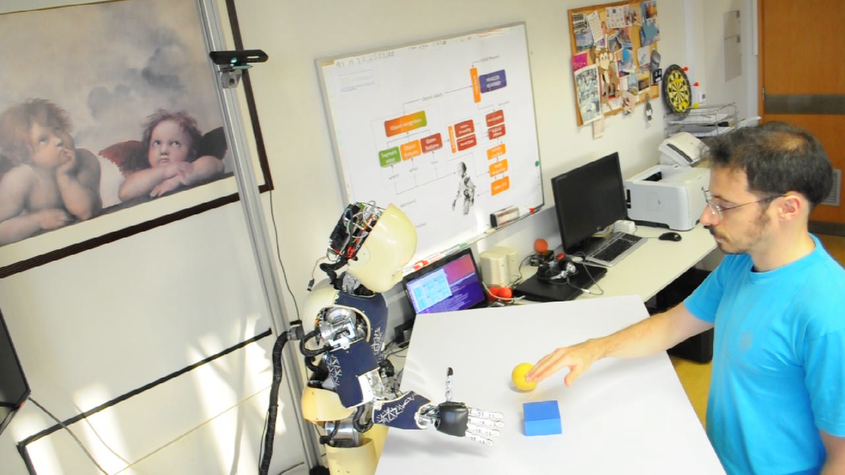
\includegraphics[width=\myWidth\linewidth]{seq2-grasp-13} } \\
%     %
%     \subfloat
%     { 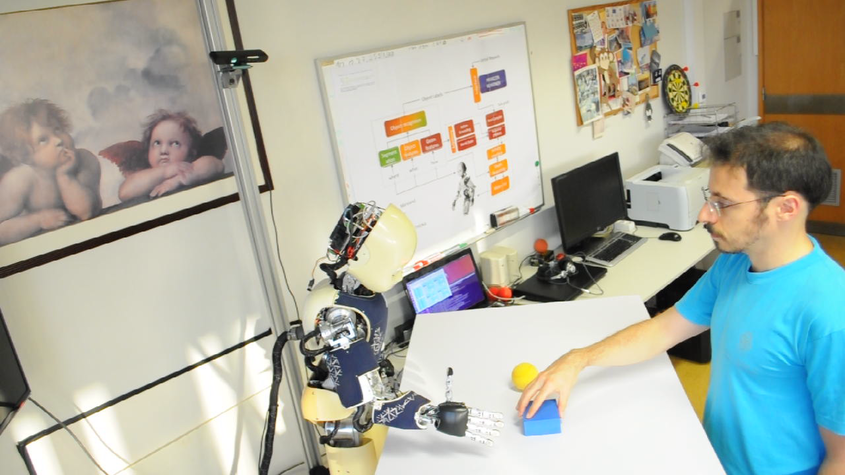
\includegraphics[width=\myWidth\linewidth]{seq2-grasp-14} } \quad
%     %
%     \subfloat
%     { 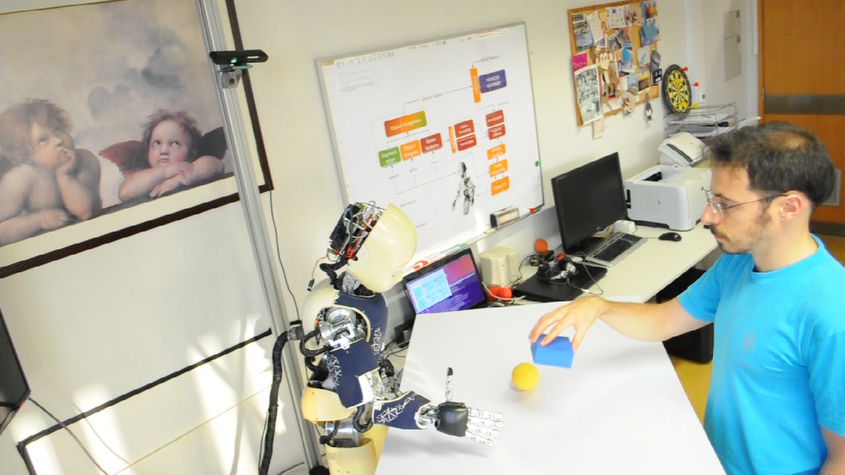
\includegraphics[width=\myWidth\linewidth]{seq2-grasp-15} } \quad
%     %
%     \subfloat
%     { 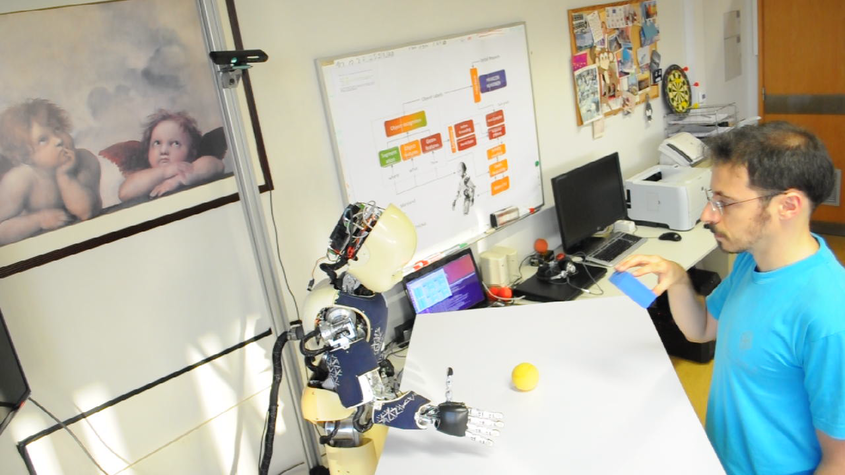
\includegraphics[width=\myWidth\linewidth]{seq2-grasp-16} }
%     \caption{grasp}
% \end{figure*}
%
% \begin{figure*}
%     \centering
%     \subfloat
%     { 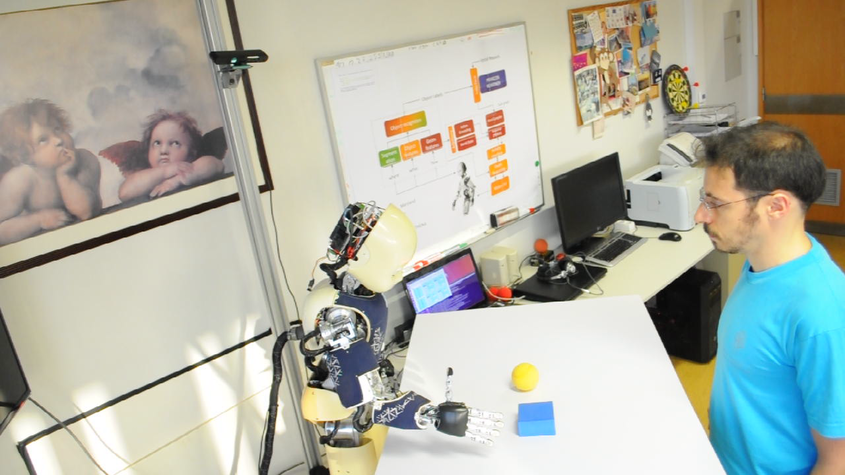
\includegraphics[width=\myWidth\linewidth]{seq2-tap-22} } \quad
%     %
%     \subfloat
%     { 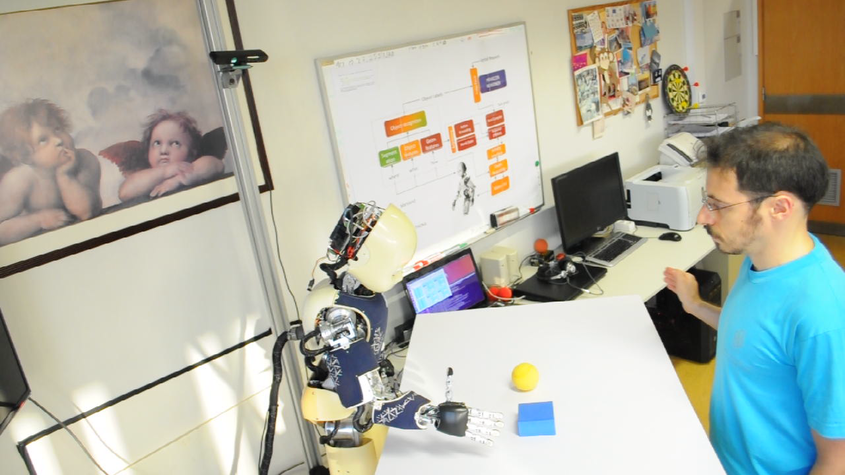
\includegraphics[width=\myWidth\linewidth]{seq2-tap-23} } \quad
%     %
%     \subfloat
%     { 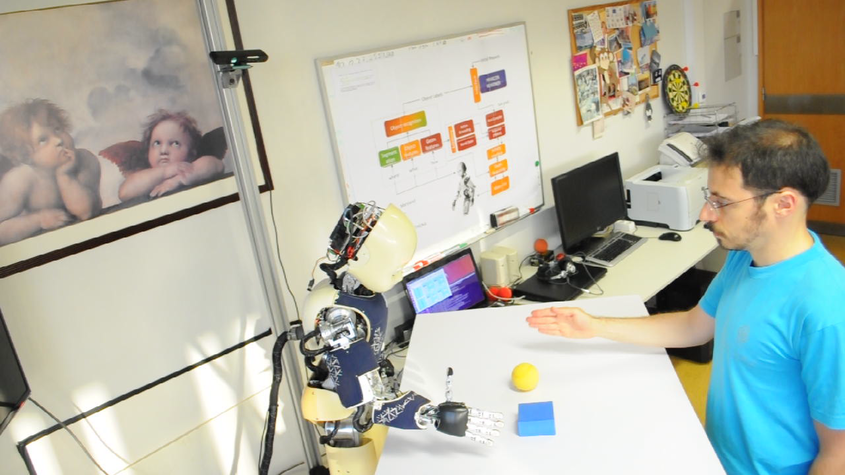
\includegraphics[width=\myWidth\linewidth]{seq2-tap-24} } \\
%     %
%     \subfloat
%     { 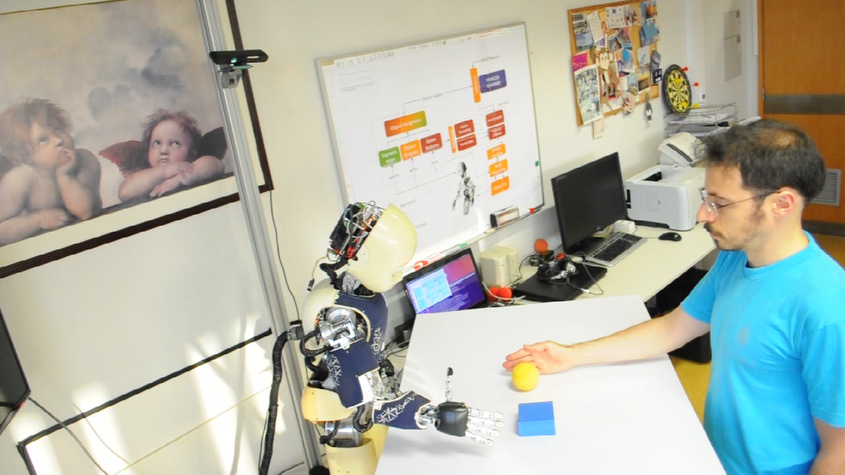
\includegraphics[width=\myWidth\linewidth]{seq2-tap-25} } \quad
%     %
%     \subfloat
%     { 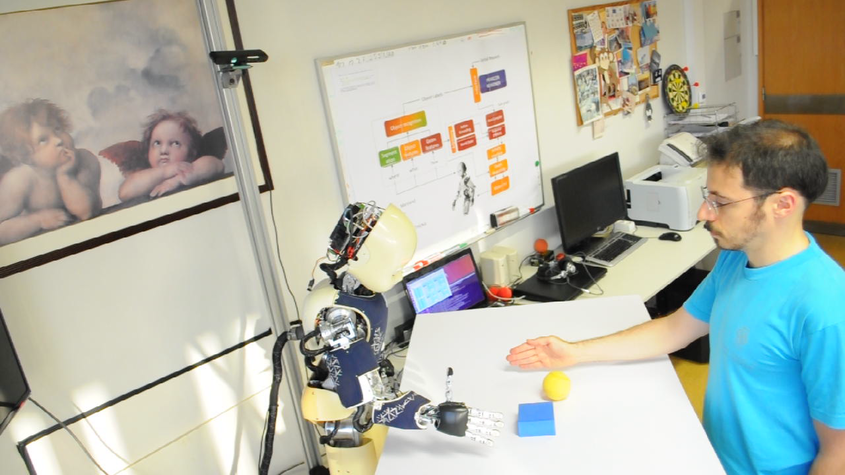
\includegraphics[width=\myWidth\linewidth]{seq2-tap-26} } \quad
%     %
%     \subfloat
%     { 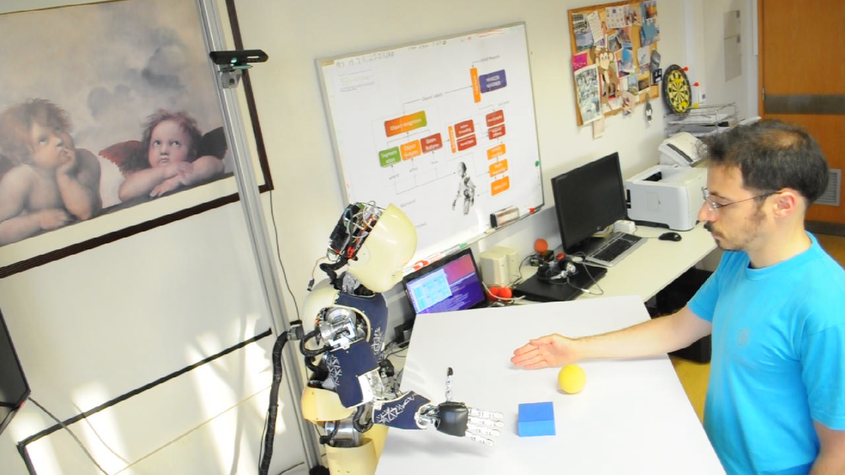
\includegraphics[width=\myWidth\linewidth]{seq2-tap-27} }
%     \caption{tap}
% \end{figure*}
%
% \begin{figure*}
%     \centering
%     \subfloat
%     { 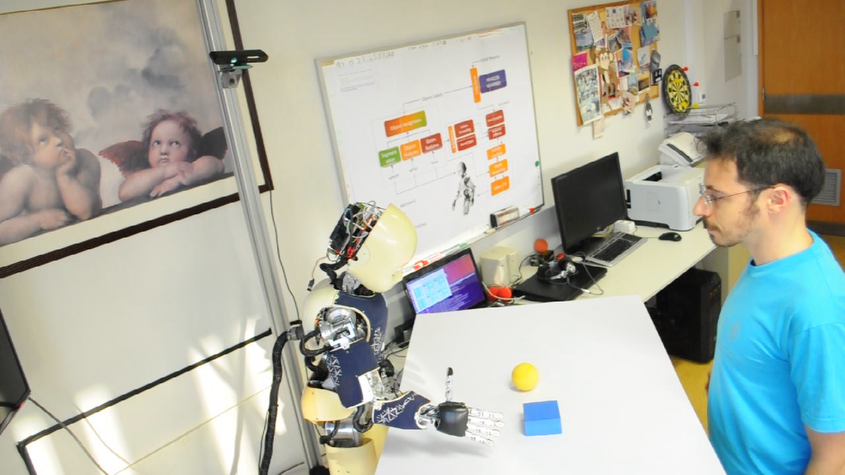
\includegraphics[width=\myWidthTwo\linewidth]{seq2-touch-2} } \quad
%     %
%     \subfloat
%     { 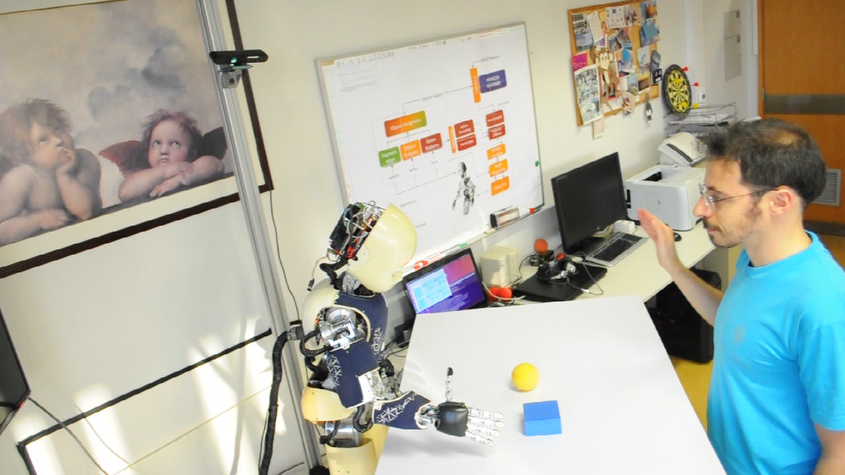
\includegraphics[width=\myWidthTwo\linewidth]{seq2-touch-3} } \quad
%     %
%     \subfloat
%     { 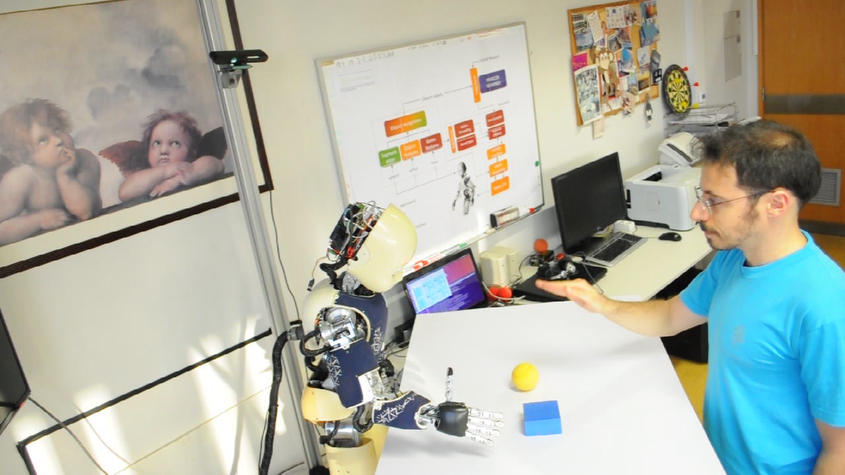
\includegraphics[width=\myWidthTwo\linewidth]{seq2-touch-4} } \quad
%     %
%     \subfloat
%     { 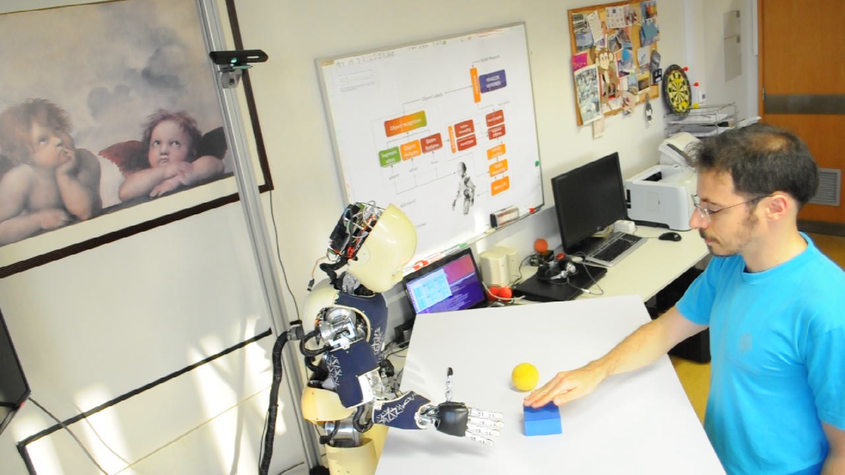
\includegraphics[width=\myWidthTwo\linewidth]{seq2-touch-5} } \\
%     %
%     \subfloat
%     { 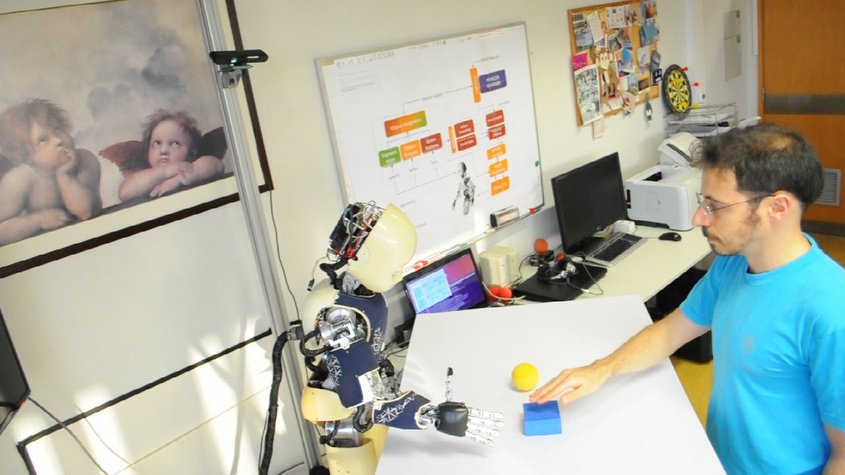
\includegraphics[width=\myWidthTwo\linewidth]{seq2-touch-6} } \quad
%     %
%     \subfloat
%     { 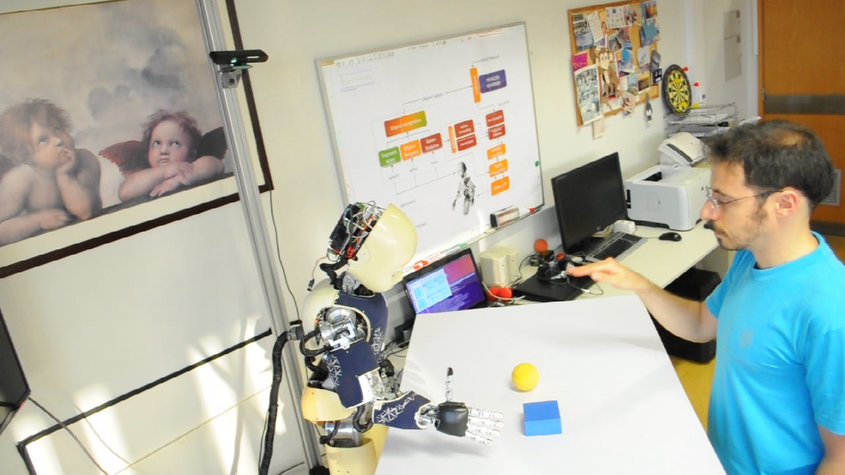
\includegraphics[width=\myWidthTwo\linewidth]{seq2-touch-7} } \quad
%     %
%     \subfloat
%     { 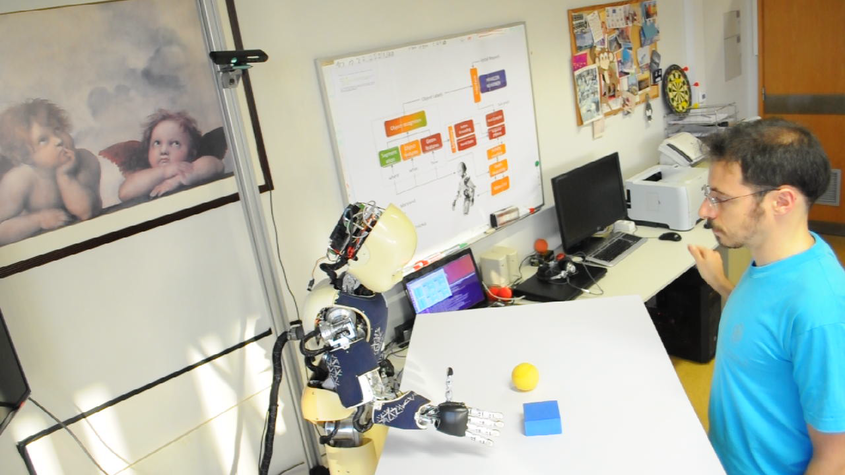
\includegraphics[width=\myWidthTwo\linewidth]{seq2-touch-8} } \quad
%     %
%     \subfloat
%     { 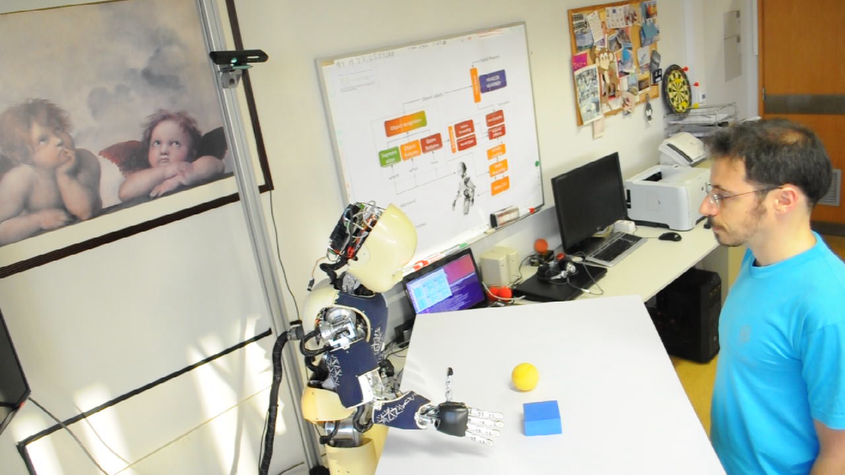
\includegraphics[width=\myWidthTwo\linewidth]{seq2-touch-9} }
%     \caption{touch}
% \end{figure*}

BELOW IS THE GLU TEXT

Robotics is progressing fast, with a steady and systematic shift from the industrial domain to domestic, public and leisure environments~\cite[ch.~65, Domestic Robotics]{siciliano:2016:handbook2}. Application areas that are particularly relevant and being researched by the scientific community include: robots for people's health and active aging, mobility, advanced manufacturing~(Industry~4.0). In short, all domains that require direct and effective \hri{} and communication (including language and gestures~\cite{matuszek:2014:aaai}).

However, robots have not reached the level of performance that would enable them to work with humans in routine activities in a flexible and adaptive way, for example in the presence of sensor noise, or unexpected events not previously seen during the training or learning phase. One of the reasons to explain this performance gap between \hh{} teamwork and a \hr{} teamwork is in the collaboration aspect, i.e., whether the members of a team understand one another. Humans have the ability of working successfully in groups. They can agree on common goals~(e.g., through verbal and non-verbal communication), work towards the execution of these goals in a coordinated way, and understand each other's physical actions~(e.g., body gestures) towards the realization of the final target. Human team coordination and mutual understanding is effective~\cite{ramnani:2004:natureneuro} because of~(i) the capacity to \emph{adapt} to unforeseen events in the environment, and re-plan one's actions in real time if necessary, and~(ii) a common motor repertoire and action model, which permits us to understand a partner's physical actions and manifested intentions as if they were our own~\cite{saponaro:2013:crhri}.

In neuroscience research, visuomotor neurons~(i.e., neurons that are activated by visual stimuli) have been a subject of ample study~\cite{rizzolatti:2001:nrn}. Mirror neurons are one class of such neurons that responds to action and object interaction, both when the agent acts and when it observes the same action performed by others, hence the name ``mirror''.

\begin{figure}
  \centering
  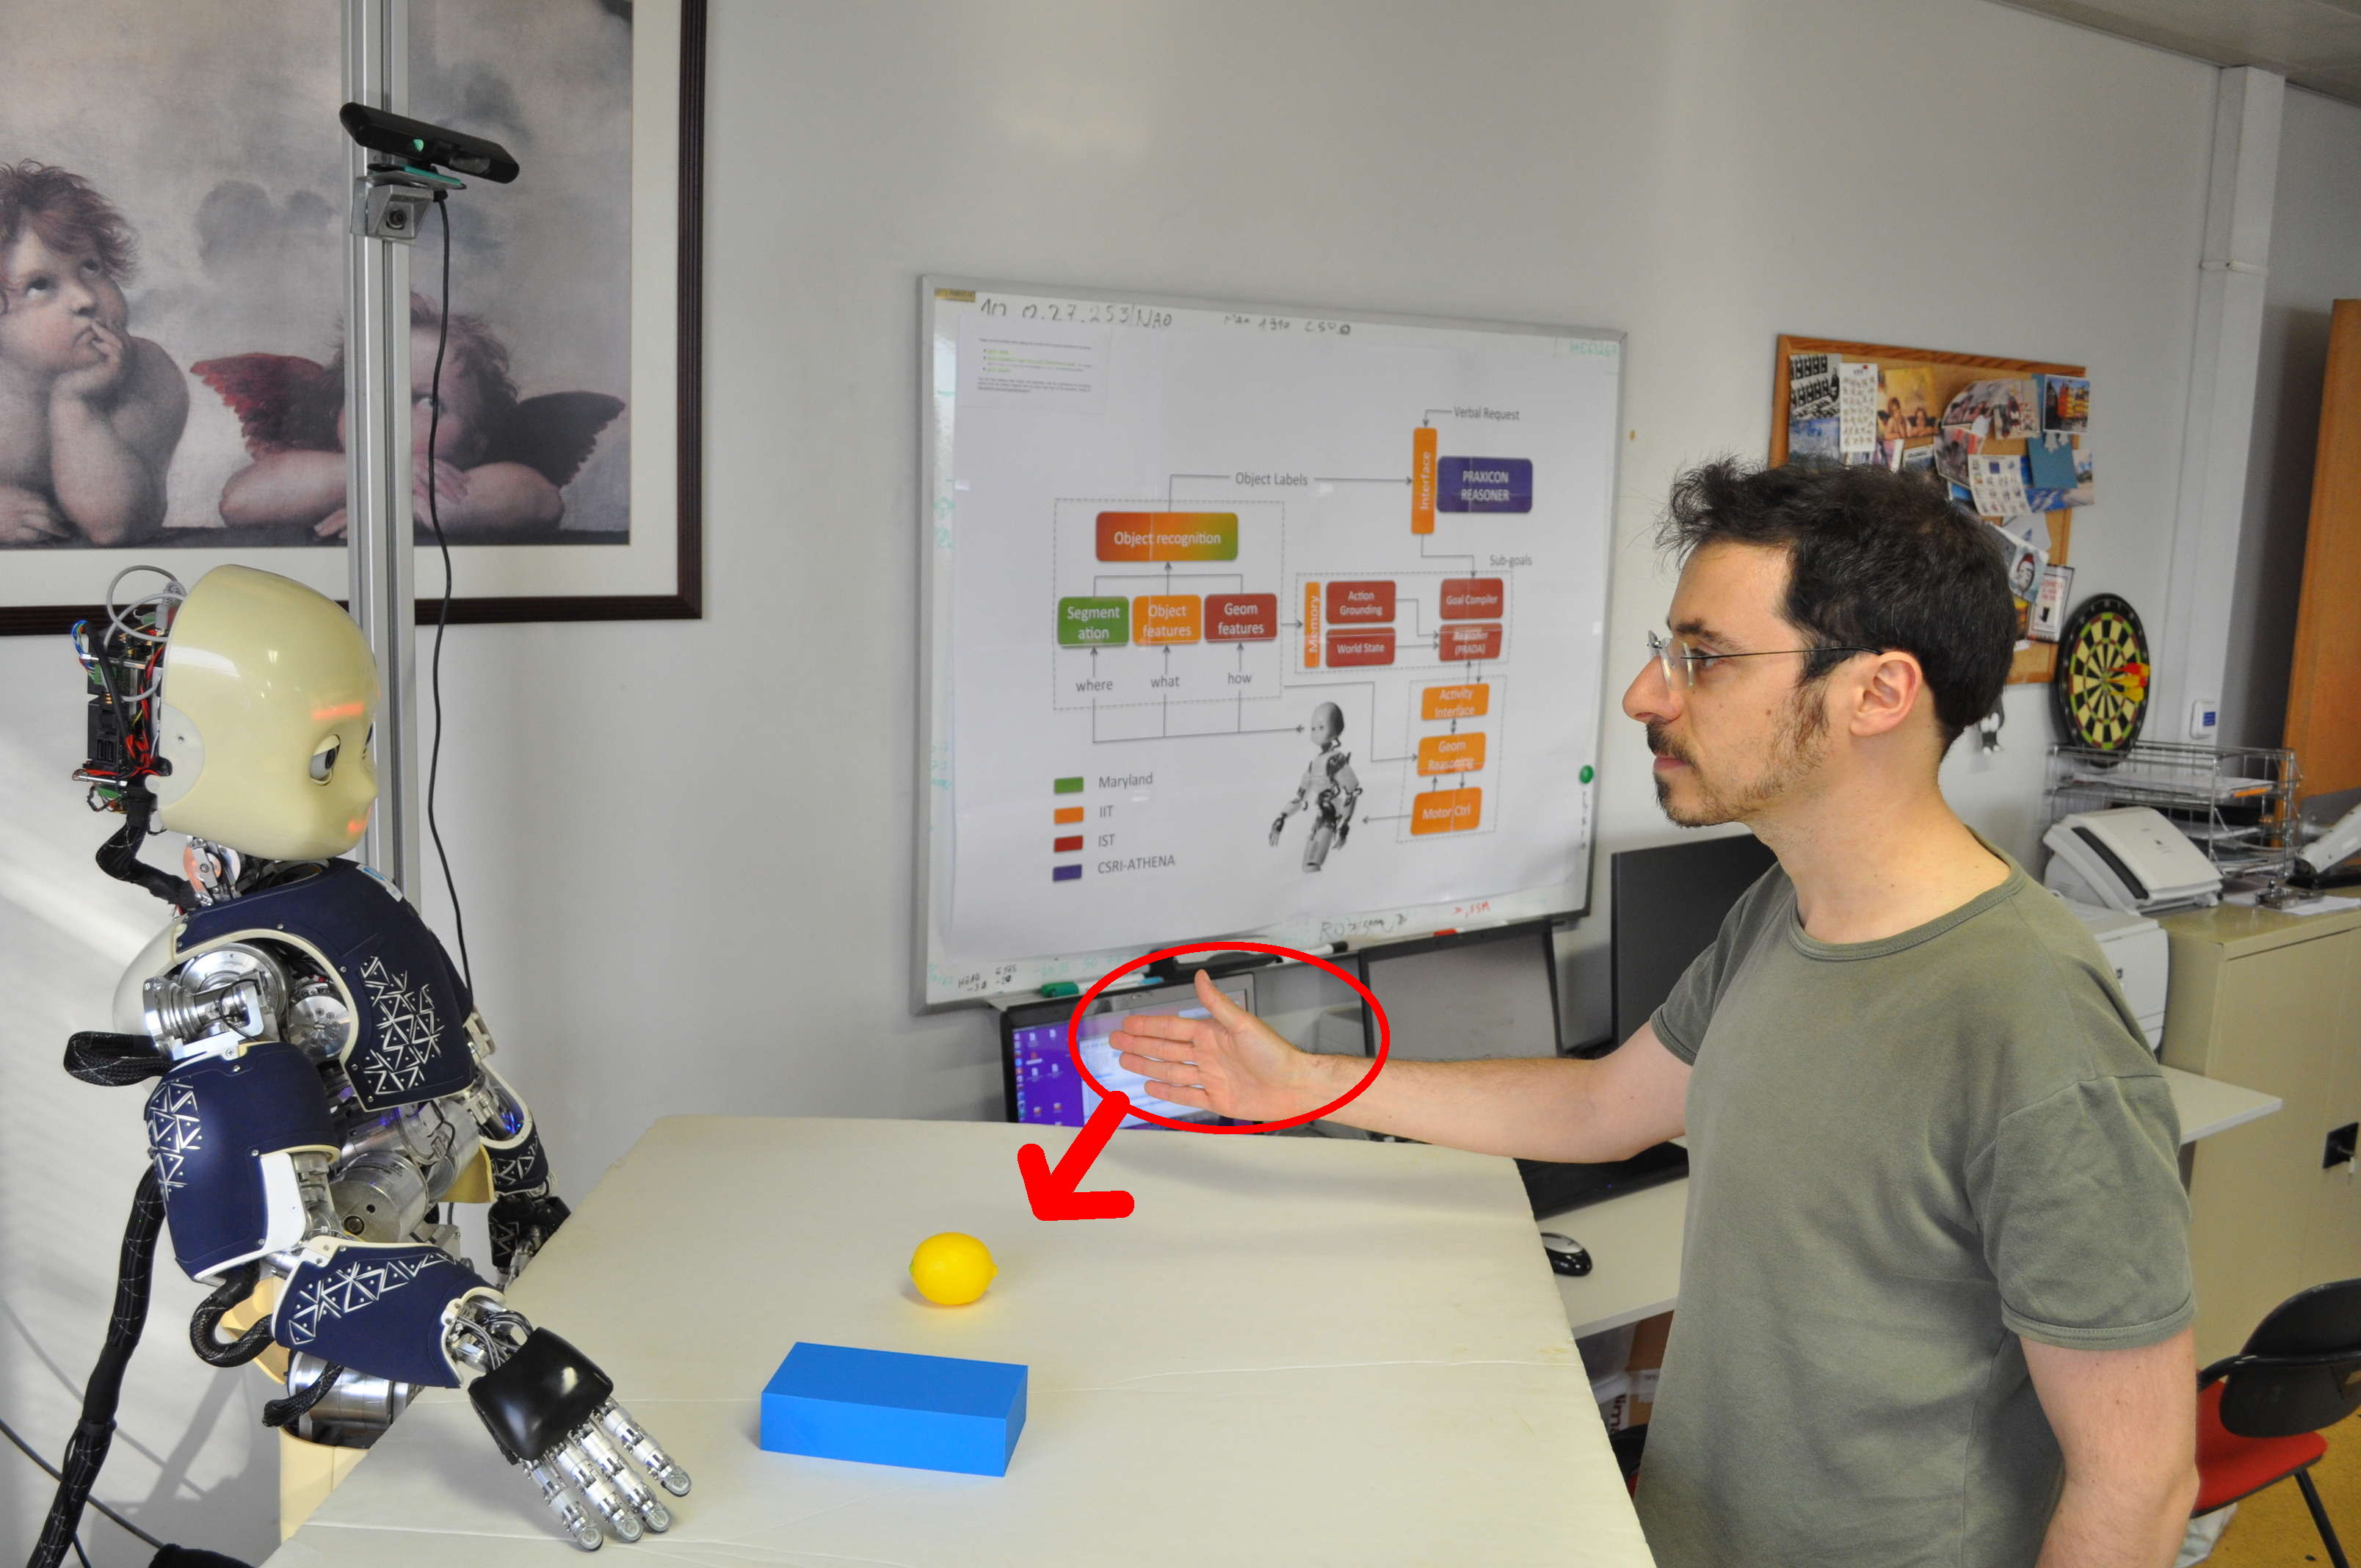
\includegraphics[width=0.9\columnwidth]{human_tap}
  \caption{Experimental setup, consisting of an iCub humanoid robot and a human user performing a manipulation gesture on a shared table with different objects on top. The depth sensor in the top-left corner is used to extract human hand coordinates for gesture recognition. Depending on the gesture and on the target object, the resulting effect will differ.}
  \label{fig:experimental_setup}
\end{figure}

This work takes inspiration from the theory of mirror neurons, and contributes towards using it on humanoid and cognitive robots. We show that a robot can first acquire knowledge by sensing and self-exploring its surrounding environment~(e.g., by interacting with available objects and building up an affordance representation of the interactions and their outcomes) and, as a result, the robot is capable of generalizing its acquired knowledge while observing another agent~(e.g., a human person) who performs similar physical actions to the ones executed during prior robot training. Fig.~\ref{fig:experimental_setup} shows the experimental setup.


TODO: ALSO CITE GLU~\cite{saponaro:2017:glu}

%%%%%%%%%%%%%%%%%%%%%%%%%%%%%%%%%%%%%%%%%%%%%%%%%%%%%%%%%%%%%%%%%%%%%%%%%%%%%%%%
%!TEX encoding = UTF-8 Unicode

\begin{figure*}
  \tikzstyle{affnode} = [ellipse, draw, thick]%fill=gray!20, thick]%node distance=1cm, text width=6em, text centered, minimum height=4em, thick]
  \tikzstyle{wordnode} = [ellipse, draw, thick]
  \tikzstyle{group} = [rectangle, draw, black, thick]%, inner sep=0.5cm
  \tikzstyle{dashedgroup} = [rectangle, draw, inner sep=0.6cm, dashed, rounded corners, black]
  \tikzstyle{dottedgrouptrapezium} = [trapezium, draw, dotted, rounded corners, black]
  \tikzstyle{affarrow} = [->, thick, >=stealth']%, shorten >=2pt]%, shorten >=2pt]
  \begin{minipage}{0.5\textwidth}
    \centering
    \begin{tikzpicture}
      % single nodes
      \node[affnode] (g1) {$g_1$};
      \node[affnode, right of=g1] (g2) {$g_2$};
      \node[right of=g2] (gdots) {$\dots$};
      \node[affnode, right of=gdots] (f1) [right=0.5cm] {$f_1$};
      \node[affnode, right of=f1] (f2) {$f_2$};
      \node[right of=f2] (fdots) {$\dots$};
      \node[affnode, below of=f1] (e2) [below=0.7cm] {$e_2$};
      \node[affnode, left of=e2] (e1) {$e_1$};
      \node[right of=e2] (edots) {$\dots$};
      \node[wordnode, below of=e1] (w1)  [below=0.7cm] {$w_1$};
      \node[wordnode, right of=w1] (w2) {$w_2$};
      \node[right of=w2] (wdots) {$\dots$};
      % groups
      \node[group, fit=(g1) (g2) (gdots),label=above:Gesture Features] (gestures) {};
      \node[group, fit=(f1) (f2) (fdots),label=above:Object Features] (features) {};
      \node[group, fit=(e1) (e2) (edots),label=above:Effects] (effects) {};
      \node[group, fit=(w1) (w2) (wdots),label=above:Words] (words) {};
      % arrows
      \draw[affarrow] (gestures) -- ([xshift=-30pt]effects.north);
      \draw[affarrow] (gestures) to [out=260,in=150] (words.west);
      \draw[affarrow] (features) -- ([xshift=20pt]effects.north);
      \draw[affarrow] ([xshift=20pt]features.south) to [out=280,in=30] (words.east);
      \draw[affarrow] ([xshift=30pt]effects.south) -- ([xshift=30pt]words.north);
      % extra
      \node[affnode, above of=gestures] (actions) [above=1cm] {Actions};
      \draw[affarrow] (actions)  to [out=220,in=90] (gestures.north west);
      \node[dashedgroup, fit=(gestures) (features) (effects) (words),label={[shift={(0:2.2)}]above:Observable variables}] (observable) {};
    \end{tikzpicture}

    \vspace{6mm}
    (a) ideal case
  \end{minipage}
  \begin{minipage}{0.5\textwidth}
    \centering
    \begin{tikzpicture}
      % single nodes
      \node[affnode] (g1) {$g_1$};
      \node[affnode, right of=g1] (g2) {$g_2$};
      \node[right of=g2] (gdots) {$\dots$};
      \node[group, fit=(g1) (g2) (gdots),label=above:Gesture Features] (gestures) {};
      \node[affnode, below of=gestures] (actions) [below=1cm] {Actions};
      \node[affnode, right of=actions] (f1) [right=1.6cm] {$f_1$};
      \node[affnode, right of=f1] (f2) {$f_2$};
      \node[right of=f2] (fdots) {$\dots$};
      \node[affnode, below of=f1] (e2) [below=0.7cm] {$e_2$};
      \node[affnode, left of=e2] (e1) {$e_1$};
      \node[right of=e2] (edots) {$\dots$};
      \node[wordnode, below of=e1] (w1)  [below=0.7cm] {$w_1$};
      \node[wordnode, right of=w1] (w2) {$w_2$};
      \node[right of=w2] (wdots) {$\dots$};
      % groups
      \node[group, fit=(f1) (f2) (fdots),label=above:Object Features] (features) {};
      \node[group, fit=(e1) (e2) (edots),label=above:Effects] (effects) {};
      \node[group, fit=(w1) (w2) (wdots),label=above:Words] (words) {};
      \node[dashedgroup, fit=(actions) (features) (effects) (words),label={[shift={(0:2.2)}]above:Affordance-word model}]{};
      % arrows
      \draw[affarrow] (actions) -- ([xshift=-30pt]effects.north);
      \draw[affarrow] (actions) to [out=260,in=150] (words.west);
      \draw[affarrow] (features) -- ([xshift=20pt]effects.north);
      \draw[affarrow] ([xshift=20pt]features.south) to [out=280,in=30] (words.east);
      \draw[affarrow] ([xshift=30pt]effects.south) -- ([xshift=30pt]words.north);
      % extra
      %\node[affnode, above of=actions] (gestures) [above=1cm] {Gesture Features};
      \draw[affarrow] (actions) -- (gestures);
      \node[dashedgroup, fit=(actions) (gestures),label=above:Gesture/Action recognition]{};
    \end{tikzpicture}

    (b) our model
  \end{minipage}
    %\centering
    %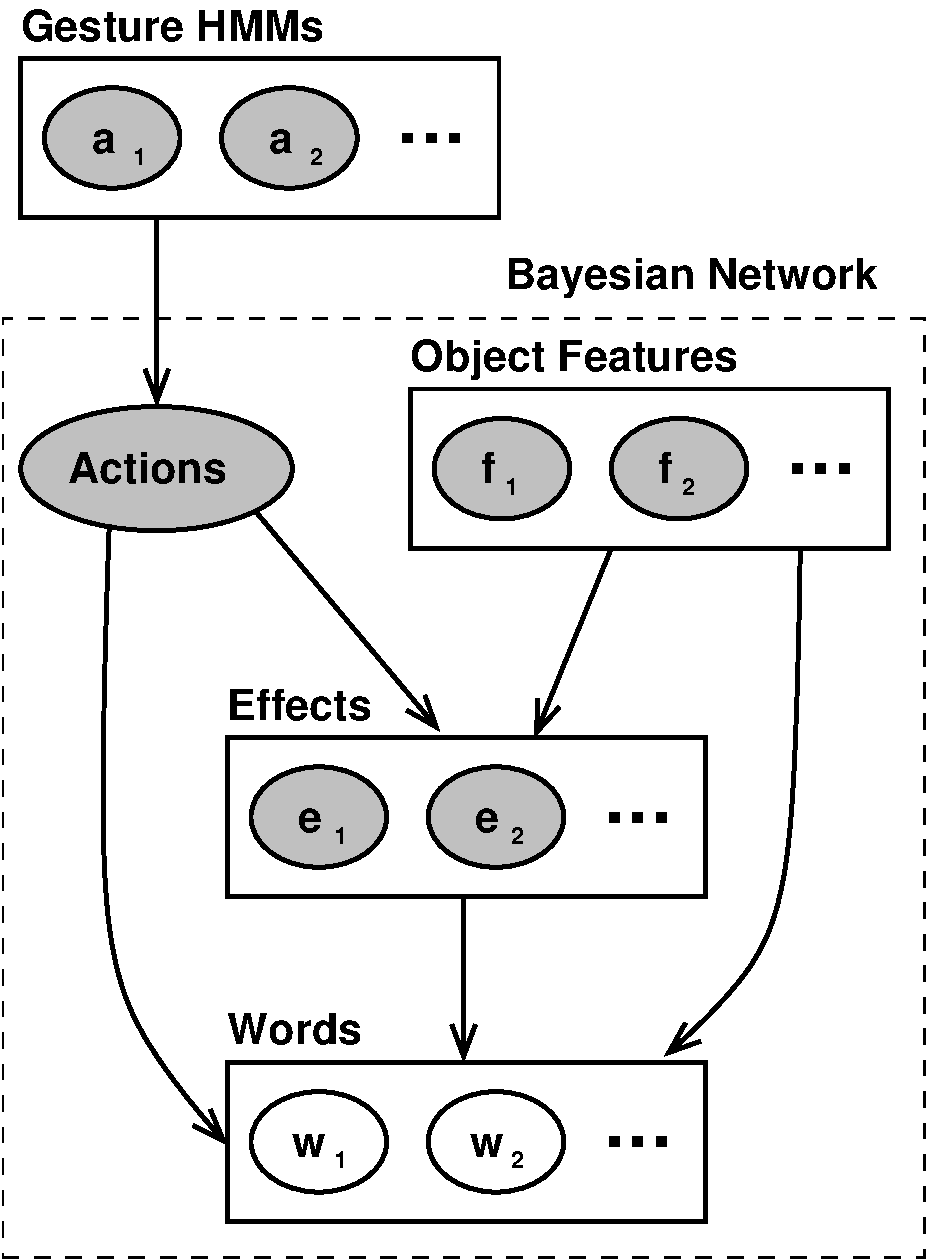
\includegraphics[width=0.8\columnwidth]{fullNetAbstract}
  \caption{Abstract representation of the probabilistic dependencies in the model. Shaded nodes are observable or measurable in the present study, and edges indicate Bayesian dependency.}
  \label{fig:model}
\end{figure*}

\section{Related Work}

BELOW IS THE GLU TEXT

A large and growing body of research is directed towards having robots learn new cognitive skills, or improving their capabilities, by interacting autonomously with their surrounding environment. In particular, robots operating in an unstructured scenario may understand available opportunities conditioned on their body, perception and sensorimotor experiences: the intersection of these elements gives rise to object affordances~(action possibilities), as they are called in psychology~\cite{gibson:2014}. The usefulness of affordances in cognitive robotics is in the fact that they capture essential properties of environment objects in terms of the actions that a robot is able to perform with them~\cite{montesano:2008,jamone:2016:tcds}.
Some authors have suggested an alternative computational model called \acp{OAC}~\cite{kruger:2011:ras}, which links low-level sensorimotor knowledge with high-level symbolic reasoning hierarchically in autonomous robots.

In addition, several works have demonstrated how combining robot affordance learning with language grounding can provide cognitive robots with new and useful skills, such as learning the association of spoken words with sensorimotor experience~\cite{salvi:2012:smcb,morse:2016:cogsci} or sensorimotor representations~\cite{stramandinoli:2016:icdl}, learning tool use capabilities~\cite{goncalves:2014:icarsc,goncalves:2014:icdl}, and carrying out complex manipulation tasks expressed in natural language instructions which require planning and reasoning~\cite{antunes:2016:icra}.

In~\cite{salvi:2012:smcb}, a joint model is proposed to learn robot affordances~(i.e., relationships between actions, objects and resulting effects) together with word meanings. The data contains robot manipulation experiments, each of them associated with a number of alternative verbal descriptions uttered by two speakers for a total of 1270~recordings. That framework assumes that the robot action is known a~priori during the training phase~(e.g., the information ``grasping'' during a grasping experiment is given), and the resulting model can be used at testing to make inferences about the environment, including estimating the most likely action, based on evidence from other pieces of information.

Several neuroscience and psychology studies build upon the theory of mirror neurons which we brought up in the Introduction. These studies indicate that perceptual input can be linked with the human action system for predicting future outcomes of actions, i.e., the effect of actions, particularly when the person possesses concrete personal experience of the actions being observed in others~\cite{aglioti:2008:basketball,knoblich:2001:psychsci}. This has also been exploited under the deep learning paradigm~\cite{kim:2017:nn}, by using a \ac{MTRNN} to have an artificial simulated agent infer human intention from joint information about object affordances and human actions. One difference between this line of research and ours is that we use real, noisy data acquired from robots and sensors to test our models, rather than virtual simulations.


%%%%%%%%%%%%%%%%%%%%%%%%%%%%%%%%%%%%%%%%%%%%%%%%%%%%%%%%%%%%%%%%%%%%%%%%%%%%%%%%
%!TEX encoding = UTF-8 Unicode

\section{Proposed Approach}

\begin{figure}
  \tikzstyle{affnode} = [ellipse, draw, thick]%fill=gray!20, thick]%node distance=1cm, text width=6em, text centered, minimum height=4em, thick]
  \tikzstyle{wordnode} = [ellipse, draw, thick]
  \tikzstyle{group} = [rectangle, draw, black, thick]%, inner sep=0.5cm
  \tikzstyle{dashedgroup} = [rectangle, draw, inner sep=0.6cm, dashed, rounded corners, black]
  \tikzstyle{dottedgrouptrapezium} = [trapezium, draw, dotted, rounded corners, black]
  \tikzstyle{affarrow} = [->, thick, >=stealth']%, shorten >=2pt]%, shorten >=2pt]
%  \centering
%  \subfloat[][Ideal case: the affordance and word variables are dependent on the detailed time-evolving description of the action.]{
%    \centering
%    \begin{tikzpicture}
%      % single nodes
%      \node[affnode] (g1) {$g_1$};
%      \node[affnode, right of=g1] (g2) {$g_2$};
%      \node[right of=g2] (gdots) {$\dots$};
%      \node[affnode, right of=gdots] (f1) [right=0.5cm] {$f_1$};
%      \node[affnode, right of=f1] (f2) {$f_2$};
%      \node[right of=f2] (fdots) {$\dots$};
%      \node[affnode, below of=f1] (e2) [below=0.7cm] {$e_2$};
%      \node[affnode, left of=e2] (e1) {$e_1$};
%      \node[right of=e2] (edots) {$\dots$};
%      \node[wordnode, below of=e1] (w1)  [below=0.7cm] {$w_1$};
%      \node[wordnode, right of=w1] (w2) {$w_2$};
%      \node[right of=w2] (wdots) {$\dots$};
%      % groups
%      \node[group, fit=(g1) (g2) (gdots),label=above:Gesture Features] (gestures) {};
%      \node[group, fit=(f1) (f2) (fdots),label=above:Object Features] (features) {};
%      \node[group, fit=(e1) (e2) (edots),label=above:Effects] (effects) {};
%      \node[group, fit=(w1) (w2) (wdots),label=above:Words] (words) {};
%      % arrows
%      \draw[affarrow] (gestures) -- ([xshift=-30pt]effects.north);
%      \draw[affarrow] (gestures) to [out=260,in=150] (words.west);
%      \draw[affarrow] (features) -- ([xshift=20pt]effects.north);
%      \draw[affarrow] ([xshift=20pt]features.south) to [out=280,in=30] (words.east);
%      \draw[affarrow] ([xshift=30pt]effects.south) -- ([xshift=30pt]words.north);
%      % extra
%      \node[affnode, above of=g1] (actions) [above=1cm] {Actions};
%      \draw[affarrow] (actions)  to [out=250,in=90] (gestures.160);
%      \node[dashedgroup, fit=(gestures) (features) (effects) (words),label={[shift={(0:2.2)}]above:Observable variables}] (observable) {};
%    \end{tikzpicture}
%    \label{fig:model:ideal}
%  } \quad\quad
  %
%  \subfloat[][Our simplified model: the affordance and word variables are dependent on the discrete action class.]{
    \centering
    \begin{tikzpicture}
      % single nodes
      \node[affnode] (g1) {$g_1$};
      \node[affnode, right of=g1] (g2) {$g_2$};
      \node[right of=g2] (gdots) {$\dots$};
      \node[group, fit=(g1) (g2) (gdots),label=above:Gesture Features] (gestures) {};
      \node[affnode, below of=gestures] (actions) [below=1cm] {Actions};
      \node[affnode, right of=actions] (f1) [right=1.6cm] {$f_1$};
      \node[affnode, right of=f1] (f2) {$f_2$};
      \node[right of=f2] (fdots) {$\dots$};
      \node[affnode, below of=f1] (e2) [below=0.7cm] {$e_2$};
      \node[affnode, left of=e2] (e1) {$e_1$};
      \node[right of=e2] (edots) {$\dots$};
      \node[wordnode, below of=e1] (w1)  [below=0.7cm] {$w_1$};
      \node[wordnode, right of=w1] (w2) {$w_2$};
      \node[right of=w2] (wdots) {$\dots$};
      % groups
      \node[group, fit=(f1) (f2) (fdots),label=above:Object Features] (features) {};
      \node[group, fit=(e1) (e2) (edots),label=above:Effects] (effects) {};
      \node[group, fit=(w1) (w2) (wdots),label=above:Words] (words) {};
      \node[dashedgroup, fit=(actions) (features) (effects) (words),label={[shift={(0:2.2)}]above:Affordance-word model}]{};
      % arrows
      \draw[affarrow] (actions) -- ([xshift=-30pt]effects.north);
      \draw[affarrow] (actions) to [out=260,in=150] (words.west);
      \draw[affarrow] (features) -- ([xshift=20pt]effects.north);
      \draw[affarrow] ([xshift=20pt]features.south) to [out=280,in=30] (words.east);
      \draw[affarrow] ([xshift=30pt]effects.south) -- ([xshift=30pt]words.north);
      % extra
      %\node[affnode, above of=actions] (gestures) [above=1cm] {Gesture Features};
      \draw[affarrow] (actions) -- (gestures);
      \node[dashedgroup, fit=(actions) (gestures),label=above:Gesture/Action recognition]{};
    \end{tikzpicture}
%    }
  \caption{Abstract representation of the probabilistic dependencies in the model.}
    \label{fig:model}
%  \label{fig:model}
\end{figure}
The purpose of the proposed approach is to model the development of language learning from a first self-centered phase to a second socially aware phase.
In the first phase the system learns by manipulating objects in its environment in a similar way as in~\cite{salvi:2012:smcb}.
In this phase, it learns to associate verbal descriptions to the combination of its actions, object properties and effects, thus grounding the meaning of words in what we call affordances.
In the second phase, the system turns to observing human actions of a similar nature as the ones explored in the first phase.
It reuses the experience acquired in the first phase to interpret the new observations and to address the correspondence problem between its own actions and the actions performed by the human.
In this phase human movements are interpreted and classified with similar methods as in~\cite{saponaro:2013:crhri}.
%reuse the experience that the robot has acquired when exploring the environment autonomously, for interpreting other people's actions.
%In order to achieve this, we combine (1)~the robot affordance model of~\cite{salvi:2012:smcb}, which associates verbal descriptions to the physical interactions of an agent with the environment, with (2)~the gesture recognition system of~\cite{saponaro:2013:crhri}, which infers the type of action from human user movements.

Figure~\ref{fig:model} illustrates the probabilistic dependencies in the complete model and will be detailed in the following subsections.
The key to our approach is the existence of the discrete variable Action, the value of which is known to the robot in the ego-centric phase of learning, but must be inferred from observation in the social phase.
In the social phase, this variable links all the other observable variables, that is, human gesture features, object properties, effect variables and words.
It allows the robot to:
\begin{itemize}
\item use language in order to determine the mapping between human and own gestures/actions, and learn the corresponding perceptual models;
\item in many cases, use the affordance variables to infer the above mapping even in the absence of a verbal descriptions;
\item once the perceptual models for human gesture/actions are acquired, use the complete model to do inference on any variable given some evidence.
\end{itemize}
In the following sections we give first details on the probabilistic models enclosed in the Affordance-word model box in Figure~\ref{fig:model}.
Then we describe the Gesture/Action recognition method.
Finally, we describe the way we combine evidence from the two models.
%We consider three \emph{manipulative gestures} corresponding to physical actions performed by agent(s) onto objects on a table~(see Fig.~\ref{fig:experimental_setup}): grasp, tap, and touch.
%Our proposed model performs probabilistic reasoning on the effects of these actions onto the objects of the world, and on the co-occurring verbal description of the experiments.

%A possible representation of the probabilistic dependencies that the robot needs to acquire in order to associate other people's actions to verbal descriptions is depicted in Fig.~\ref{fig:model:ideal}.
%The intended actions result in movements of the body that can be measured in terms of \emph{gesture features}.
%These movements, in turn, may determine some \emph{effects} on the surroundings, expressed by a number of relevant measurable variables.
%Those effects are also determined by the particular \emph{object features} associated with the objects that are involved in the action and that are also observable.
%Finally, an observer composes a verbal description of the situation based on all the observable variables.
%
%By combining the affordance model in \cite{salvi:2012:smcb} and the gesture recognition system in \cite{saponaro:2013:crhri}, however, we need to do some simplifying assumptions, that are depicted in Fig.~\ref{fig:model:our}.
%The main difference is that, in the learning phase in \cite{salvi:2012:smcb}, the intended action was known to the robot.
%The robot could, therefore, learn direct dependencies between the actions and the other variables in the \affwords{} model depicted in the corresponding dashed box in Fig.~\ref{fig:model:our}.
%Although some of the effect variables refer to the robot's arm movements, this information was not rich enough to recognize each particular gesture and could therefore not be used directly to interpret other people's behavior.
%
%This limitation can be partly overcome by the gesture/action recognition model of~\cite{saponaro:2013:crhri}, which can recover the particular intended action from the gesture features.
%Consequently, the relationship between Gesture Features, Object Features, Effects and Words, that we described earlier, is mediated by the Actions variable in our model.
%The combination of the two models is our main contribution, and allows us to relax the assumption made in \cite{salvi:2012:smcb} that the action is known during the learning phase.
%
%In the remainder of this section, we give details about the \affwords{} model, about the gesture/action recognition model employed in the study, and about the method that we employ to perform probabilistic inference by merging the information provided by those two models.

%BELOW IS THE GLU TEXT

%In this paper, we combine (1)~the robot affordance model of~\cite{salvi:2012:smcb}, which associates verbal descriptions to the physical interactions of an agent with the environment, with (2)~the gesture recognition system of~\cite{saponaro:2013:crhri}, which infers the type of action from human user movements.
%We consider three \emph{manipulative gestures} corresponding to physical actions performed by agent(s) onto objects on a table~(see Fig.~\ref{fig:experimental_setup}): grasp, tap, and touch.
%We reason on the effects of these actions onto the objects of the world, and on the co-occurring verbal description of the experiments. In the complete framework, we will use \acfp{BN}, which are a probabilistic model that represents random variables and conditional dependencies on a graph, such as in Fig.~\ref{fig:model}. One of the advantages of using \acp{BN} is that their expressive power allows the marginalization over any set of variables given any other set of variables.

%Our main contribution is that of extending~\cite{salvi:2012:smcb} by relaxing the assumption that the action is known during the learning phase.
%This assumption is acceptable when the robot learns through self-exploration and interaction with the environment, but must be relaxed if the robot needs to generalize the acquired knowledge through the observation of another~(human) agent.
%We estimate the action performed by a human user during a \hr{} collaborative task, by employing statistical inference methods and \acp{HMM}. This provides two advantages. First, we can infer the executed action during training. Secondly, at testing time we can merge the action information obtained from gesture recognition with the information about affordances.

\subsection{\AffWords{} Modeling}
\label{sec:bn}
Following the method adopted in~\cite{salvi:2012:smcb}, we use a Bayesian probabilistic framework to allow a robot to ground the basic world behavior and verbal descriptions associated to it.
All variables in the model are discrete or are discretized from continuous sensory variables through clustering in a preliminary learning phase.
Details on the variable definition and possible values are given in Table~\ref{tab:bnsymb}.
Note that the name of the values have been assigned by us arbitrarily to the clusters, for the sake of making the results more human-interpretable.
However, the robot has no prior knowledge about the meaning of these clusters.

\begin{table}
    \centering
    \caption{The symbolic variables of the \acl{BN} (from~\cite{salvi:2012:smcb}), with the corresponding discrete values obtained from clustering during robot exploration of the environment.}
    \label{tab:bnsymb}
    %\begin{tabular}{clp{2.7cm}p{2.5cm}}
    \begin{tabular}{cp{3.3cm}l}
    \toprule
    symbol & description     & values \\
    \midrule
    $a$ & action          & grasp, tap, touch \\
    \midrule
    $f_1$ & object color   & blue, yellow, green1, green2 \\
    $f_2$ & object size     & small, medium, big \\
    $f_3$ & object shape    & sphere, box \\
    \midrule
    $e_1$ & object velocity & slow, medium, fast \\
    $e_2$ & robot hand velocity & slow, fast \\
    $e_3$ & relative object hand velocity & slow, medium, fast \\
    $e_4$ & object hand contact & short, long \\
    \midrule
    $w_1$--$w_{49}$ & presence of each word in the verbal description & binary \\
    \bottomrule
    \end{tabular}
\end{table}

To simplify the notation, we can group the affordance and word variables according to their use for the following descriptions: action variable~$A = \{a\}$, object feature variables~$F=\{f_1, f_2, \dots\}$, effect variables~$E=\{e_1, e_2, \dots\}$ and word variables~$W = \{w_1, w_2, \dots\}$.
The \ac{BN} model relates all these variables by means of the joint probability distribution~$P(A, F, E, W)$, sketched by the Affordance-word model box in Fig.~\ref{fig:model}.
The dependency structure and the model parameters are estimated by the robot in an ego-centric way through interaction with the environment, as in~\cite{salvi:2012:smcb}.
As a consequence, during learning, the robot knows what action it is performing with certainty, and the variable~$A$ assumes a deterministic value.
During inference, the probability distribution on the variable~$A$ can be inferred from evidence on the other nodes.
For example, if the robot is asked to make a spherical object roll, it will be able to select the action tap as most likely to obtain the desired effect, based on previous experience.
%This assumption is relaxed in the present study, by extending the model to the observation of external~(human) agents as explained below.


\newcommand{\myscalefactor}{0.8}

\newcommand{\standardhmm}[1]{
    \node[draw,circle] (hmm#1s1) {$s_1$};
    \node[draw,circle, right of=hmm#1s1] (hmm#1s2) {$s_2$};
    \node[circle, right of=hmm#1s2] (hmm#1s3) {\dots};
    \node[draw,circle, right of=hmm#1s3] (hmm#1s4) {$s_Q$};
    \node[left of=hmm#1s1]  (invisible1) {};
    \node[right of=hmm#1s4] (invisible2) {};
    \path[->] (hmm#1s1) edge (hmm#1s2);
    \path[loop above] (hmm#1s1) edge (hmm#1s1);
    \path[->] (hmm#1s2) edge (hmm#1s3);
    \path[loop above] (hmm#1s2) edge (hmm#1s2);
    \path[dashed] (hmm#1s2) -- (hmm#1s3);
    \path[->] (hmm#1s3) edge (hmm#1s4);
    \path[loop above] (hmm#1s4) edge (hmm#1s4);
    %\path[->] (hmm#1s4) edge[bend left] (hmm#1s1);
    \path[->] (invisible1) edge (hmm#1s1);
    \path[->] (hmm#1s4) edge (invisible2);
}

\newcommand{\modeltwo}{
  \begin{tikzpicture}[scale=\myscalefactor, every node/.style={scale=\myscalefactor}]
  \matrix (M) [matrix of nodes, ampersand replacement=\&] {%
    grasp gesture HMM \& \standardhmm{1} \\
    tap gesture HMM \& \standardhmm{2} \\
    touch gesture HMM \& \standardhmm{3} \\
    %garbage \& \standardhmm{4} \\
  };
  \end{tikzpicture}
}

\begin{figure}
  \centering
  \modeltwo
  \caption{Structure of the \acp{HMM} used for human gesture recognition, adapted from~\cite{saponaro:2013:crhri}. In this work, we consider three independent, multiple-state \acp{HMM}, each of them trained to recognize one of the considered manipulation gestures.}
  \label{fig:hmms}
\end{figure}

\subsection{Gesture/Action Recognition}
When observing a human performing actions, the value of the action variable~$A$ is not known to the robot neither during learning nor during inference.
During learning, we assume that the robot has yet not acquired a perceptual model of the gestures associated to the human actions.
The value of~$A$ can, however, be inferred either from a verbal description of the scene or from the other affordance nodes through the affordance-word model described earlier.

For example, similarly to the previous section, the affordance-word model predicts that performing a tap action on a spherical object will result in high velocity of the object.
If the human performs an unknown action on a spherical object and obtains a high velocity, the robot will be able to infer that the action is most probably a tap, although it was not able to recognize the gesture associated with this action.

This information can be used to train a gesture/action recognition system similar to the one in~\cite{saponaro:2013:crhri}.
The system, depicted in Fig.~\ref{fig:hmms} and corresponding to the Gesture/Action recognition block in Fig.~\ref{fig:model}, is based on hidden Markov models with Gaussian emitting probability distributions.
%The gesture recognition models are represented in Fig.~\ref{fig:hmms}, and correspond to the Gesture/Action recognition block in Fig.~\ref{fig:model}.
%As for the gesture recognition \acsp{HMM}, we use the models that we previously trained in~\cite{saponaro:2013:crhri} for spotting the manipulation-related gestures under consideration.
Our input features are the 3D coordinates of the tracked human hand indicated by the $g_i$ variables in Fig.~\ref{fig:model}.
The coordinates are obtained with a commodity depth sensor, then transformed to be centered on the person torso~(to be invariant to the distance of the user from the sensor) and normalized to account for variability in amplitude~(to be invariant to wide/emphatic vs narrow/subtle executions of the same gesture class).

The model for each gesture/action is a so-called left-to-right \ac{HMM}, where the transition model between the discrete states~$\mathcal{S} = \{s_1, \dots, s_Q\}$ is structured so that states with lower index represent events that occur earlier in time.
%set of (hidden) discrete states~$\mathcal{S} = \{s_1, \dots, s_Q\}$ which model the temporal phases comprising the dynamic execution of the gesture, and by a set of parameters~$\lambda = \{ A, B, \Pi \}$, where~$A = \{ a_{ij} \}$ is the transition probability matrix, $a_{ij}$ is the transition probability from state~$s_i$ at time~$t$ to state~$s_j$ at time~$t+1$, $B = \{ f_i \}$ is the set of $Q$~observation probability functions~(one per state~$i$) with continuous mixtures of Gaussian values, and~$\Pi$ is the initial probability distribution for the states.

Although not expressed so far in the notation, the continuous variables~$g_i$ are measured at regular time intervals.
At a certain time step~$n$, the feature vector can be expressed as~$\mathbf{g}[n] = \{g_1[n], \dots, g_D[n]\}$.
The input to the model is a sequence of~$N$ such feature vectors~$\mathbf{g}[1], \dots, \mathbf{g}[N]$ that we call for simplicity~$G_1^N$, where~$N$ can vary for every recording.

At recognition~(testing) time, we can use the models to estimate the likelihood of a new sequence of observations~$G_1^N$, given each possible gesture/action by means of the \FB{} inference algorithm.
%We can express this likelihood as $\mathcal{L}_\text{HMM}(G_1^N \given A)$, where $a$ is one of the possible actions.
We can express this likelihood as $\mathcal{L}_\text{HMM}(G_1^N \given A=a)$, where $a$ is one of the possible actions.
By normalizing the likelihoods, assuming that the gestures are equally likely \emph{a priori}, we can obtain the posterior probability of the action given the sequence of observations that we call~$\phmm(A \given G_1^N)$.

%In Sec.~\ref{sec:combination}, we discuss different ways in which the output information of the gesture recognizer can be combined with the \acl{BN} of words and affordances.

\subsection{Combining the \acs{BN} with Gesture \acsp{HMM}}
\label{sec:combination}
Once learned, the two models described above define two probability distributions over the relevant variables for the problem:
$\pbn(A, F, E, W)$ and~$\phmm(A \given G_1^N)$.
The goal during inference is to merge the information provided by both models and estimate~$\pcomb(A, F, E, W \given G_1^N)$, that is, the joint probability of all the affordance and word variables, given that we observe a certain gesture/action performed by the human.

To simplify the notation, we call $X = \{A, F, E, W\}$ the set of affordance and word variables~$\{a, f_1, f_2, \dots, e_1, e_2, \dots, w_1, w_2, \dots\}$.
During inference, we have a (possibly empty) set of observed variables~$\xobs \subseteq X$, and a set of variables $\xinf \subseteq X$ on which we wish to perform the inference.
In order for the inference to be non-trivial it must be~$\xobs \cap \xinf = \varnothing$, that is, we should not observe any inference variable.
According to the \ac{BN} alone, the inference will compute the probability distribution of the inference variables~$\xinf$ given the observed variables~$\xobs$ by marginalizing over all the other (latent) variables $\xlat = X \setminus (\xobs \cup \xinf)$, where~$\setminus$~is the set difference operation:
\begin{eqnarray*}
 \pbn(\xinf \given \xobs) = \sum_{\xlat} \pbn(\xinf, \xlat \given \xobs).
\end{eqnarray*}

If we want to combine the evidence brought by the \ac{BN} with the evidence brought by the hidden Markov model, there are two cases that can occur:
\begin{enumerate}
\item the variable action is included among the inference variables: $A \in \xinf$, or

\item the variable action is not included among the inference variables: $A \in \xlat$.
\end{enumerate}

Here, we are excluding the case where we observe the action directly~($A\in \xobs$) for two reasons: firstly, this would correspond to the robot performing the action itself, whereas we are interested in interpreting other people's actions;
secondly, this would make the evidence on the gesture features $G_1^N$ irrelevant, because in the model in Fig.~\ref{fig:model}, there is a tail-to-tail connection from $G_1^N$ to the rest of the variables through the action variable, which means that, given the action, all dependencies to the gesture features are dropped.

The two cases enumerated above can be addressed separately when we do inference.
In the first case, we call~$\xinf^\prime$ the set of inference variables excluding the action~$A$, that is, $\xinf = \{\xinf^\prime, A\}$.
We can write:
\begin{align*}
  & \pcomb(\xinf \given  \xobs, G_1^N) = \pcomb(A, \xinf^\prime \given  \xobs, G_1^N)= \\
  &= \sum_{\xlat} \pcomb(A, \xinf^\prime, \xlat \given \xobs, G_1^N)=\\
  &= \sum_{\xlat} \left[\pbn(A, \xinf^\prime, \xlat \given \xobs, G_1^N)\right. \\[-4mm]
    & \mspace{80mu} \left.\phmm(A, \xinf^\prime, \xlat \given \xobs, G_1^N)\right]= \\
  &= \left[\sum_{\xlat} \pbn(A, \xinf^\prime, \xlat \given \xobs)\right] \phmm(A \given G_1^N) \\
  &= \pbn(\xinf \given \xobs) \phmm(A \given G_1^N).
\end{align*}
This means that we can evaluate the two models independently and multiply the distribution we obtain from the \ac{BN} over all the possible value of the inference variables, by the \ac{HMM} posterior for the corresponding value of the action.

In the second case, where the action is among the latent variables, we define, similarly, $\xlat = \{A, \xlat^\prime\}$, and we have:
\begin{align*}
  & \pcomb(\xinf \given \xobs, G_1^N) = \\
  &= \sum_{\{A,\xlat^\prime\}} \pcomb(\xinf, A, \xlat^\prime \given \xobs, G_1^N)=\\
  &= \sum_{\{A,\xlat^\prime\}} \left[\pbn(\xinf, A, \xlat^\prime \given \xobs, G_1^N)\right. \\[-4mm]
    & \mspace{100mu} \left.\phmm(\xinf, A, \xlat^\prime \given \xobs, G_1^N)\right]= \\[2mm]
  &= \sum_{\{A,\xlat^\prime\}} \left[\pbn(\xinf, A, \xlat^\prime \given \xobs) \phmm(A \given G_1^N)\right] \\
  &= \sum_{A}\left[\phmm(A \given G_1^N)\sum_{\xlat^\prime} \pbn(\xinf, A, \xlat^\prime \given \xobs)\right] \\
  &= \sum_{A}\left[\phmm(A \given G_1^N) \pbn(\xinf, A \given \xobs)\right]. \\
\end{align*}
This time, we first need to use the \ac{BN} to do inference on the inference variables~$\xinf$ and the action variable~$A$, and then marginalize out~$A$ after having multiplied the probabilities by the \ac{HMM} posterior.

%GLU TEXT
%
%In this study we wish to generalize the model of~\cite{salvi:2012:smcb} by observing external~(human) agents, as shown in Fig.~\ref{fig:experimental_setup}. For this reason, the full model is now extended with a perception module capable of inferring the action of the agent from visual inputs. This corresponds to the Gesture \acp{HMM} block in Fig.~\ref{fig:model}. The \AffWords{} \acf{BN} model and the Gestures \acp{HMM} may be combined in different ways~\cite{pan:2006:ictai}:
%\begin{enumerate}
%\item the Gesture \acp{HMM} may provide a hard decision on the action performed by the human~(i.e., considering only the top result) to the \ac{BN},
%
%\item the Gesture \acp{HMM} may provide a posterior distribution~(i.e., soft decision) to the \ac{BN},
%
%\item if the task is to infer the action, the posterior from the Gesture \acp{HMM} and the one from the \ac{BN} may be combined as follows, assuming that they provide independent information:
%\begin{equation*}
%p(A) = \phmm(A) \, \pbn(A).
%\end{equation*}
%\end{enumerate}
%
In the experimental section, we will show that what the robot has learned subjectively or alone~(by self-exploration, knowing the action identity as a prior~\cite{salvi:2012:smcb}), can subsequently be used when observing a new agent~(human), provided that the actions can be estimated with Gesture \acp{HMM} as in~\cite{saponaro:2013:crhri}.


%%%%%%%%%%%%%%%%%%%%%%%%%%%%%%%%%%%%%%%%%%%%%%%%%%%%%%%%%%%%%%%%%%%%%%%%%%%%%%%%
%!TEX encoding = UTF-8 Unicode

\section{Experimental Results}

BELOW IS THE GLU TEXT

\begin{figure}
    \centering
    \subfloat[][Prediction of the movement effect on a small sphere.]
    { 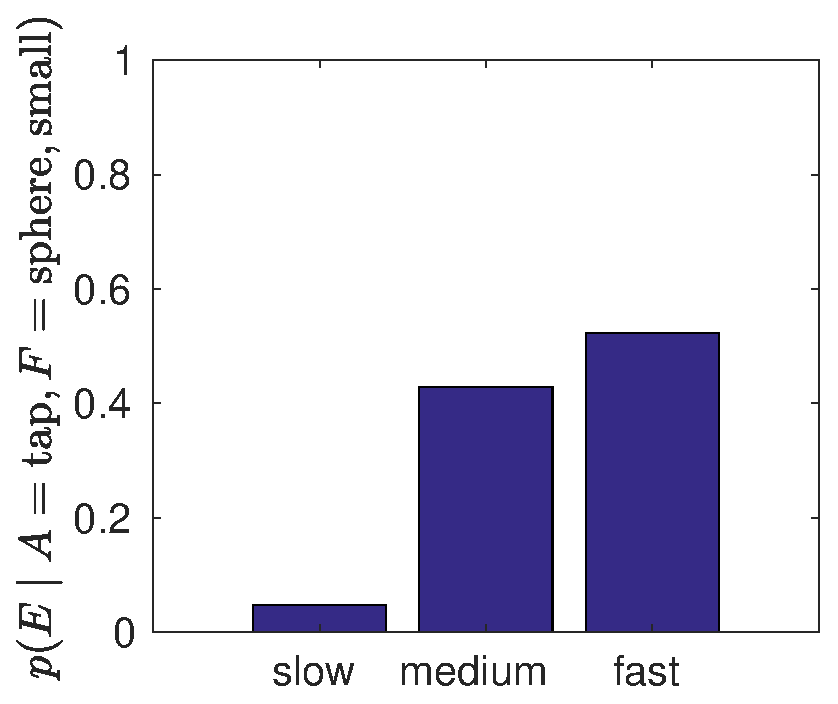
\includegraphics[width=0.45\linewidth]{effectpred_sphere.eps} \label{fig:effect_pred:sphere} } \quad
    %
    \subfloat[][Prediction of the movement effect on a big box.]
    { 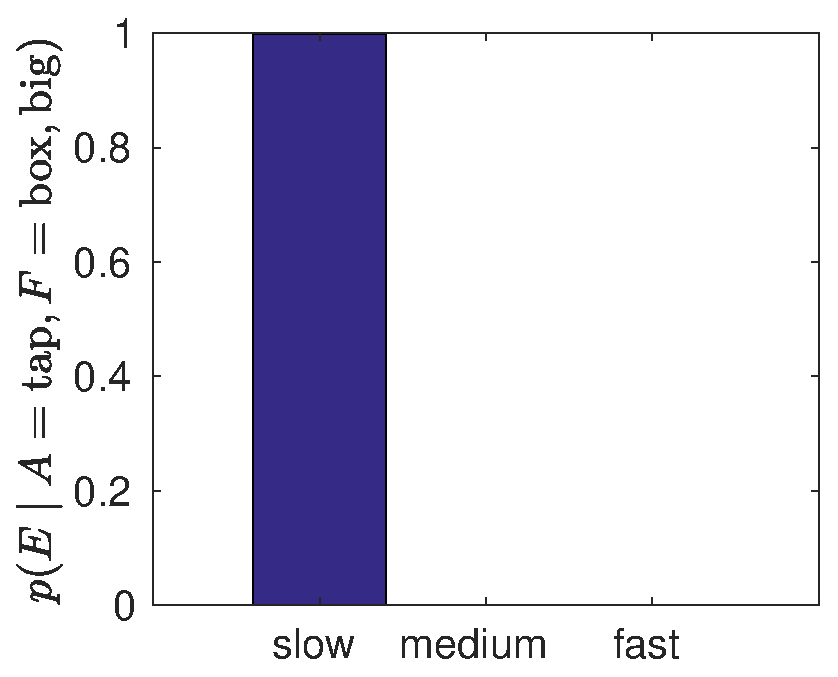
\includegraphics[width=0.45\linewidth]{effectpred_box.eps} \label{fig:effect_pred:box} }
    \caption{Object velocity predictions, given prior information~(from Gesture \acp{HMM}) that the human user performs a tapping action.}
    \label{fig:effect_pred}
\end{figure}

We present preliminary examples of two types of results: predictions over the effects of actions onto environment objects, and predictions over the associated word descriptions in the presence or absence of an action prior. In this section, we assume that the Gesture \acp{HMM} provide the discrete value of the recognized action performed by a human agent~(i.e., we enforce a hard decision over the observed action, referring to the possible combination strategies listed in Sec.~\ref{sec:combination}).

\subsection{Effect Prediction}

From our combined model of words, affordances and observed actions, we report the inferred posterior value of the Object Velocity effect, given prior information about the action~(provided by the Gesture \acp{HMM}) and also about object features~(Shape and Size). Fig.~\ref{fig:effect_pred} shows the computed predictions in two cases. Fig.~\ref{fig:effect_pred:sphere} shows the anticipated object velocity when the human user performs the tapping action onto a small spherical object, whereas Fig.~\ref{fig:effect_pred:box} displays it when the target object is a big box. Indeed, given the same observed action prior~(lateral tap on the object), the expected movement is very different depending on the physical properties of the target object.

\begin{figure}
\centering
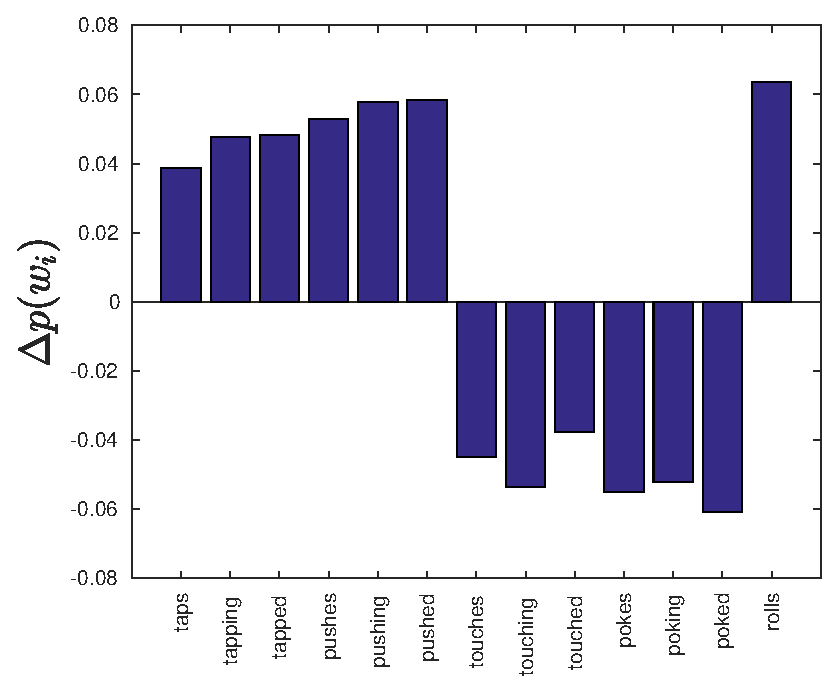
\includegraphics[width=0.9\columnwidth]{partialfig.eps}
\caption{Variation of word occurrence probabilities: $\Delta p(w_i) = p(w_i \mid F, E, A=\text{tap}) - p(w_i \mid F,E)$, where $F = \{\text{Size=big, Shape=sphere}\}$, $E = \{\text{ObjVel=fast}\}$. This variation corresponds to the difference of word probability when we add the tap action evidence~(obtained from the Gesture \acp{HMM}) to the initial evidence about object features and effects. We have omitted words for which no significant variation was observed.}
\label{fig:probdiff}
\end{figure}

\subsection{Prediction of Words}

In this experiment, we compare the associated \emph{verbal description} obtained by the \acl{BN} in the absence of an action prior, with the ones obtained in the presence of one. In particular, we compare the \emph{probability of word occurrence} in the following two situations:
\begin{enumerate}
\item when the robot prior knowledge~(evidence in the \ac{BN}) includes information about object features and effects only: \emph{Size=big, Shape=sphere, ObjVel=fast};

\item when the robot prior knowledge includes, in addition to the above, evidence about the action as observed from the Gestures \acp{HMM}: \emph{Action=tap}.
\end{enumerate}

Fig.~\ref{fig:probdiff} shows the variation in word occurrence probabilities between the two cases, where we have omitted words for which no significant variation was observed in this case. We can interpret the difference in the predictions as follows:
\begin{itemize}
\item as expected, the probabilities of words related to tapping and pushing increase when a tapping action evidence from the Gestures \acp{HMM} is introduced; conversely, the probabilities of other action words~(touching and poking) decreases;

\item interestingly, the probability of the word \emph{rolling}~(which is an effect of an action onto an object) also increases when the tapping action evidence is entered. Even though the initial evidence of case~$1$ already included some effect information~(the velocity of the object), it is only now, when the robot perceives that the physical action was a tap, that the event rolling is associated.
\end{itemize}


%%%%%%%%%%%%%%%%%%%%%%%%%%%%%%%%%%%%%%%%%%%%%%%%%%%%%%%%%%%%%%%%%%%%%%%%%%%%%%%%
%!TEX encoding = UTF-8 Unicode

\section{Conclusions and Future Work}

Things we need to discuss:
\begin{itemize}
\item the effect variables in the BN include hand velocity. How does this relate to the gesture features in the HMM? Can we learn the connection?
\item in order to achieve the ideal case in Figure~\ref{fig:model} we would need to learn the complex relationship between hand movements and affordance variables:
  \begin{itemize}
  \item how can this be achieved in the ego-centric learning? Mixture of HMMs and BN? Would it be possible to learn the dependency structure in this complex model?
  \item assuming it is possible to learn in the ego-centric way, how can this be extended to the other agent? Coordinates will definitely be different. In the current study we could directly map the two because we were using the categorical variable ``action''.
  \end{itemize}
\end{itemize}

BELOW IS THE GLU TEXT

Within the scope of cognitive robots that operate in unstructured environments, we have discussed a model that combines word affordance learning with body gesture recognition. We have proposed such an approach, based on the intuition that a robot can generalize its previously-acquired knowledge of the world~(objects, actions, effects, verbal descriptions) to the cases when it observes a human agent performing familiar actions in a shared \hr{} environment. We have shown promising preliminary results that indicate that a robot's ability to predict the future can benefit from incorporate the knowledge of a partner's action, facilitating scene interpretation and, as a result, teamwork.

In terms of future work, there are several avenues to explore. The main ones are (i)~the implementation of a fully probabilistic fusion between the affordance and the gesture components~(e.g., the soft decision discussed in Sec.~\ref{sec:combination}); (ii)~to run quantitative tests on larger corpora of \hr{} data; (iii)~to explicitly address the correspondence problem of actions between two agents operating on the same world objects~(e.g., a pulling action from the perspective of the human corresponds to a pushing action from the perspective of the robot, generating specular effects).


%%%%%%%%%%%%%%%%%%%%%%%%%%%%%%%%%%%%%%%%%%%%%%%%%%%%%%%%%%%%%%%%%%%%%%%%%%%%%%%%
\section*{Acknowledgments}

This work was partially supported by the FCT project~UID/EEA/50009/2013 and by the CHIST-ERA project IGLU.

%%%%%%%%%%%%%%%%%%%%%%%%%%%%%%%%%%%%%%%%%%%%%%%%%%%%%%%%%%%%%%%%%%%%%%%%%%%%%%%%
\printbibliography

\end{document}
